\begin{frame}
   \frametitle{Talk Outline}
   \begin{tikzpicture}[font=\small]
      \tikzset{>=latex} % arrow heads
      \draw[step=1,black!15,very thin,opacity=\gridopacity] (0,0) grid (12,8);

      \node[fill=blue!15,minimum width=11cm] at (6,7.5) {\strut What to Optimize?};

      \node[fill=black!3,minimum width=5cm,minimum height=3cm] (utility) at (3.25,5.6) {};
      \node[anchor=north] at (utility.north) {\strut Maximizing Utility};
      \node at (3.25,5.35) {\includegraphics[width=2.5cm]{build/pvx-utility-anytime}};

      \node[fill=black!3,minimum width=5cm,minimum height=3cm] (family) at (8.75,5.6) {};
      \node[anchor=north] at (family.north) {\strut Utility in C-Space Familes};
      \node at (8.75,5.4) {\includegraphics[width=3.0cm]{build/multiple-sets}};

      \node[fill=blue!15,minimum width=11cm] at (6,3.5) {\strut How to Optimize?};

      \node[fill=black!3,minimum width=5cm,minimum height=3cm] (lazysp) at (3.25,1.6) {};
      \node[anchor=north] at (lazysp.north) {\strut Lazy Pathfinding};
      \node[draw=black!30,fill=white,inner sep=5pt] at (3.25,1.4) {
         \includegraphics[width=3.8cm]{build/lazysp-icon}};

      \node[fill=black!3,minimum width=5cm,minimum height=3cm] (ibid) at (8.75,1.6) {};
      \node[anchor=north] at (ibid.north) {\strut Dynamic Pathfinding};
      \node[draw=black!30,inner sep=0pt] at (8.75,1.4) {
         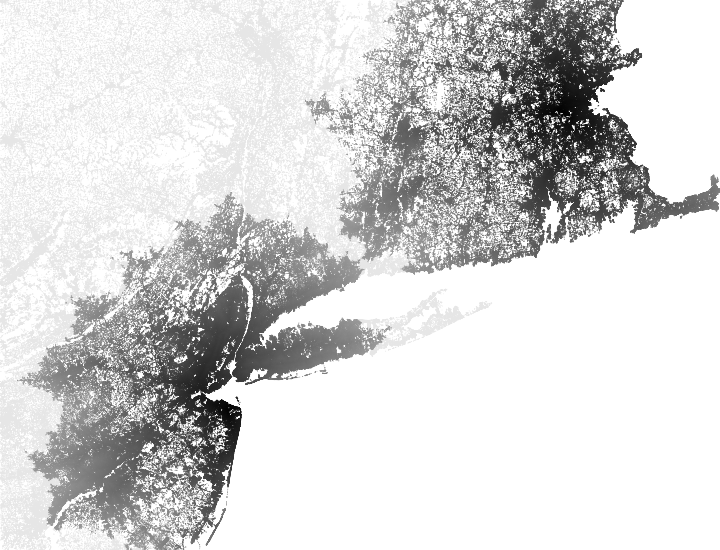
\includegraphics[width=2.9cm]{figs/incbi-road-ne/singleshot/example-bidijkstra.png}};

      \only<2>
      {
         \draw[ultra thick] (lazysp.north east) rectangle (lazysp.south west);
      }
      
   \end{tikzpicture}
\end{frame}

%\begin{frame}
%   \frametitle{Pathfinding on Graphs}
%   
%   The \emph{shortest-path problem} is prevalent and fundamental.
%   
%   Lots of applications.
%   
%   Graph $G=(V,E)$, edge weight function $w: E \rightarrow \mathbb{R}$.
%   
%   Single-pair, all-pairs, single-source/single-sink, etc.
%   
%   Bounded-suboptimal, incremental, anytime, etc ...
%\end{frame}

%\iffalse

\begin{frame}
   \frametitle{Motivation: The Shortest Path (SP) Problem}
   \begin{tikzpicture}[font=\small]
      \tikzset{>=latex} % arrow heads
   
      \draw[step=1,black!15,very thin,opacity=\gridopacity] (0,0) grid (12,8);
      
      \only<2->{
         \node at (1,7) {
\includegraphics[width=1.5cm]{figs/rubik.png}};
         \node at (3,7) {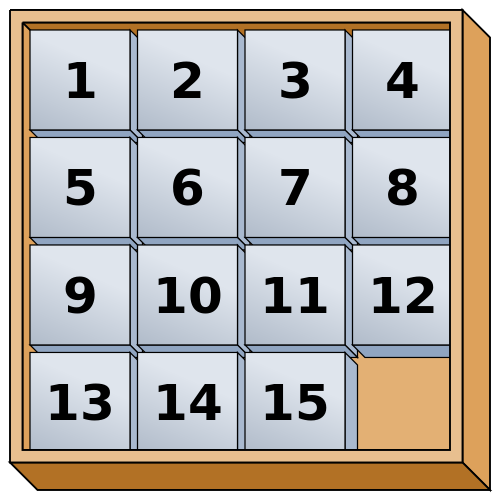
\includegraphics[width=1.5cm]{figs/15puzzle.png}};
      }
      \only<3->{
         \node at (5,7) {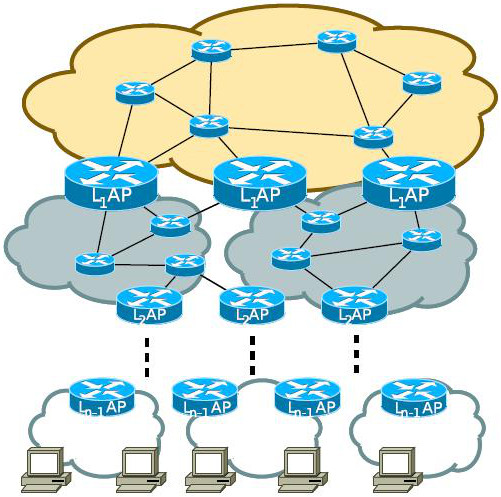
\includegraphics[width=1.5cm]{figs/internet-routers.jpg}};
      }
      \only<4->{
         \node at (7,7) {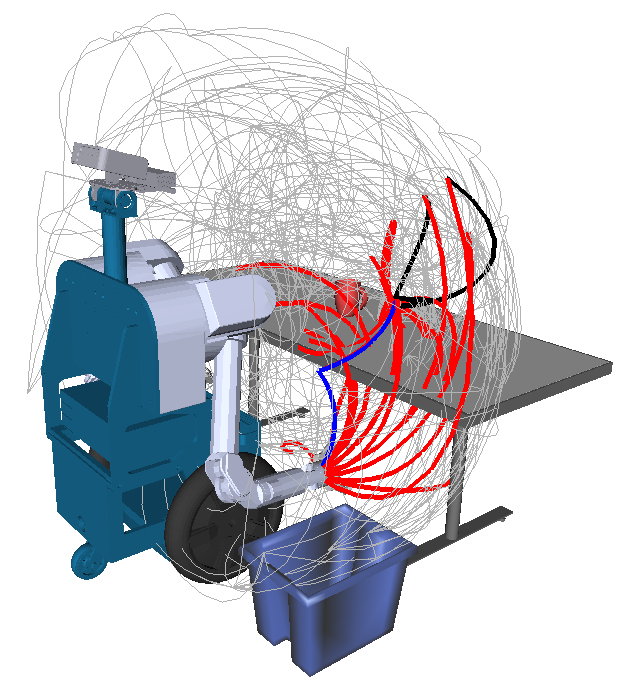
\includegraphics[width=1.5cm]{figs/lazysp-herbarm/herbarm-path33.png}};
         \node at (9,7) {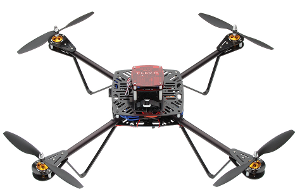
\includegraphics[width=1.5cm]{figs/quad.png}};
      }
      \only<5->{
         \node at (11,7) {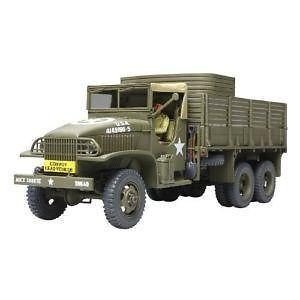
\includegraphics[width=1.5cm]{figs/military-truck.jpg}};
      }
      
      \only<6->{
         % graph
         
         \coordinate (va) at ( 2.0,4.0);
         \coordinate (vb) at ( 3.5,4.7);
         \coordinate (vc) at ( 4.0,5.9);
         \coordinate (vd) at ( 5.5,4.5);
         \coordinate (ve) at ( 8.0,5.0);
         \coordinate (vf) at (10.0,4.0);
         \coordinate (vg) at ( 1.5,5.0);
         \coordinate (vh) at ( 4.0,3.5);
         \coordinate (vi) at ( 7.0,3.2);
         \coordinate (vj) at ( 6.5,5.5);
         \coordinate (vk) at ( 9.0,3.5);
         
         \only<9->{
            \node[circle,fill=black!20,inner sep=0.1cm] at (va) {};
            \node[circle,fill=black!20,inner sep=0.1cm] at (vf) {};
         }
         
         \only<10->{
            \draw[line width=0.2cm,color=black!30,line cap=round]
               (va) -- (vb) -- (vd) -- (ve) -- (vf);
         }
         
         \node[circle,fill=black,inner sep=0.05cm] at (va) {};
         \node[circle,fill=black,inner sep=0.05cm] at (vb) {};
         \node[circle,fill=black,inner sep=0.05cm] at (vc) {};
         \node[circle,fill=black,inner sep=0.05cm] at (vd) {};
         \node[circle,fill=black,inner sep=0.05cm] at (ve) {};
         \node[circle,fill=black,inner sep=0.05cm] at (vf) {};
         \node[circle,fill=black,inner sep=0.05cm] at (vg) {};
         \node[circle,fill=black,inner sep=0.05cm] at (vh) {};
         \node[circle,fill=black,inner sep=0.05cm] at (vi) {};
         \node[circle,fill=black,inner sep=0.05cm] at (vj) {};
         \node[circle,fill=black,inner sep=0.05cm] at (vk) {};
         
         \draw (va) -- (vb) coordinate [midway] (eab);
         \draw (vb) -- (vc) coordinate [midway] (ebc);
         \draw (vb) -- (vd) coordinate [midway] (ebd);
         \draw (vc) -- (vd) coordinate [midway] (ecd);
         \draw (vd) -- (ve) coordinate [midway] (ede);
         \draw (ve) -- (vf) coordinate [midway] (eef);
         \draw (va) -- (vg) coordinate [midway] (eag);
         \draw (vb) -- (vg) coordinate [midway] (ebg);
         \draw (va) -- (vh) coordinate [midway] (eah);
         \draw (vd) -- (vh) coordinate [midway] (edh);
         \draw (vb) -- (vh) coordinate [midway] (ebh);
         \draw (vd) -- (vi) coordinate [midway] (edi);
         \draw (ve) -- (vi) coordinate [midway] (eei);
         \draw (vc) -- (vj) coordinate [midway] (ecj);
         \draw (vd) -- (vj) coordinate [midway] (edj);
         \draw (ve) -- (vj) coordinate [midway] (eej);
         \draw (vf) -- (vk) coordinate [midway] (efk);
         \draw (vi) -- (vk) coordinate [midway] (eik);
         \draw (ve) -- (vk) coordinate [midway] (eek);
         
         \only<7->{
            \node[circle,inner sep=0.02cm,fill=white,opacity=0.9,font=\scriptsize] at (eab) {5};
            \node[circle,inner sep=0.02cm,fill=white,opacity=0.9,font=\scriptsize] at (ebc) {5};
            \node[circle,inner sep=0.02cm,fill=white,opacity=0.9,font=\scriptsize] at (ebd) {6};
            \node[circle,inner sep=0.02cm,fill=white,opacity=0.9,font=\scriptsize] at (ecd) {7};
            \node[circle,inner sep=0.02cm,fill=white,opacity=0.9,font=\scriptsize] at (ede) {9};
            \node[circle,inner sep=0.02cm,fill=white,opacity=0.9,font=\scriptsize] at (eef) {7};
            \node[circle,inner sep=0.02cm,fill=white,opacity=0.9,font=\scriptsize] at (eag) {3};
            \node[circle,inner sep=0.02cm,fill=white,opacity=0.9,font=\scriptsize] at (ebg) {6};
            \node[circle,inner sep=0.02cm,fill=white,opacity=0.9,font=\scriptsize] at (eah) {6};
            \node[circle,inner sep=0.02cm,fill=white,opacity=0.9,font=\scriptsize] at (edh) {7};
            \node[circle,inner sep=0.02cm,fill=white,opacity=0.9,font=\scriptsize] at (ebh) {5};
            \node[circle,inner sep=0.02cm,fill=white,opacity=0.9,font=\scriptsize] at (edi) {8};
            \node[circle,inner sep=0.02cm,fill=white,opacity=0.9,font=\scriptsize] at (eei) {8};
            \node[circle,inner sep=0.02cm,fill=white,opacity=0.9,font=\scriptsize] at (ecj) {8};
            \node[circle,inner sep=0.02cm,fill=white,opacity=0.9,font=\scriptsize] at (edj) {6};
            \node[circle,inner sep=0.02cm,fill=white,opacity=0.9,font=\scriptsize] at (eej) {4};
            \node[circle,inner sep=0.02cm,fill=white,opacity=0.9,font=\scriptsize] at (efk) {3};
            \node[circle,inner sep=0.02cm,fill=white,opacity=0.9,font=\scriptsize] at (eik) {6};
            \node[circle,inner sep=0.02cm,fill=white,opacity=0.9,font=\scriptsize] at (eek) {6};
         }
      }
      
      \only<6->{
         \node[draw,align=center,minimum height=1.0cm,minimum width=2.9cm,thick]
            at (4.0,2.05) {Graph\\$G=(V,E)$};
      }
      \only<7->{
         \node[draw,align=center,minimum height=1.0cm,minimum width=2.9cm,thick]
            at (8.0,2.05) {Weight Function\\$w:E \rightarrow \mathbb{R}$};
         %\node[align=center,color=black!50] at (10.75,2) {
         %   $w(e) \geq 0$\\
         %   $w(e) > 0$\\
         %   $w(e) \geq w_{\ms{est}}(e)$\\
         %};
      }
      \only<8->{
         \node[draw,align=center,minimum height=1.0cm,minimum width=4cm,thick]
            (alg) at (6,0.55) {Shortest Path\\Algorithm};
         \draw[->] (4.5,1.55) -- (4.5,1.05);
         \draw[->] (7.5,1.55) -- (7.5,1.05);
      }
      \only<9->{
         \node[draw,align=center,shape=document,minimum width=3.0cm,ultra thin]
            (query) at (2,0.55) {Query $v_s$, $v_t$\;\;};
         \draw[->] (query.east) -- (alg.west);
         \node[left=0.1cm of va] {$v_s$};
         \node[right=0.1cm of vf] {$v_t$};
      }
      \only<10->{
         \node[draw,align=center,shape=document,minimum width=2.0cm,ultra thin]
            (path) at (10,0.55) {Path $p^*$\;};
         \draw[->] (alg.east) -- (path.west);
      }
      
   \end{tikzpicture}
\end{frame}

% application     -> graph representation    -> algorithm      -> path -> application solution
% [ lots of them]    G=(V,E)                    [lots of them]
%                    w: e -> R
%                    root vertices (v_s, v_t)
%                    (vertex heuristic?)
%                    problem
%                    - single-pair
%                    - optimal
%                    - bounded-suboptimal
%                    - bounded-cost
 
%\begin{frame}
%   \frametitle{Pathfinding on Graphs 2}
%   \begin{tikzpicture}
%      \tikzset{>=latex} % arrow heads
%   
%      \draw[step=1,black!15,very thin,opacity=\gridopacity] (0,0) grid (12,8);
%      
%      \node at (1.5,7.5) {Applications};
%      
%      \node at (1.0,6.5) {
\includegraphics[width=1.5cm]{figs/rubik.png}};
%      \node at (2.0,6.5) {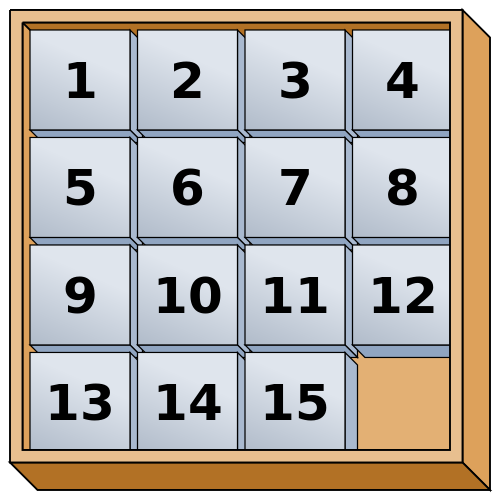
\includegraphics[width=1.5cm]{figs/15puzzle.png}};
%      \node at (1.5,4.5) {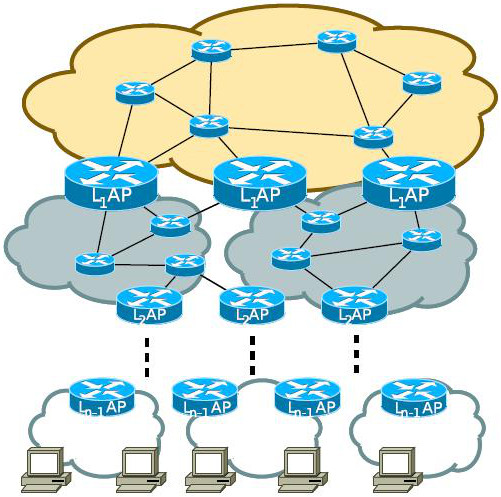
\includegraphics[width=1.5cm]{figs/internet-routers.jpg}};
%      \node at (1.5,3.0) {Traffic Routing};
%      \node at (1.5,2.5) {Motion Planning};
%      %\node at (1.5,2.0) {Optimal Motion Planning};
%      
%      \node at (6.0,7.5) {Representation};
%      
%      \node at (10.5,7.5) {Algorithms};
%      
%      \node[align=center] at (7,3) {
%         $w(e) \geq 0$\\
%         $w(e) > 0$\\
%         $w(e) \geq w_{\ms{est}}(e)$\\
%      };
%      
%      %\draw[step=1cm,black!10,very thin] (0,0) grid (8,4);
%      \node[draw,align=center,minimum height=1.0cm,thick]
%         at (6.0,6.0) {Graph\\$G=(V,E)$};
%      \node[draw,align=center,minimum height=1.0cm,thick]
%         at (6.0,4.5) {Weight Function\\$w:E \rightarrow [0,+\infty]$};
%      \node[draw,align=center,shape=document,minimum width=3.0cm,ultra thin]
%         (query) at (6,1) {Query $v_s$, $v_t$\;\;};
%      
%      \node at (10.5,6.5) {Dijkstra's};
%      \node at (10.5,5.5) {A*};
%      \node at (10.5,4.5) {IDA*};
%      \node at (10.5,3.5) {PEA*};
%      
%   \end{tikzpicture}
%\end{frame}

\begin{frame}
   \frametitle{Motivation: The Shortest Path (SP) Problem}
   \begin{tikzpicture}[font=\small]
      \tikzset{>=latex} % arrow heads
      
      \draw[step=1,black!15,very thin,opacity=\gridopacity] (0,0) grid (12,8);
   
      % c-space obstacles
      \only<8-12>{
         \fill[black!20] (4.5,3.25) rectangle (6.0,5.0);
         \fill[black!20] (8.5,4.00) rectangle (9.5,5.5);
         \only<8-10>{
            \node[color=black!70,font=\scriptsize] at (5.25,3.5) {$CO_1$};
            \node[color=black!70,font=\scriptsize] at (9.0,5.25) {$CO_2$};
         }
         \only<11->{
            \node[color=black!70,font=\scriptsize] at (5.25,3.5) {$SO_1$};
            \node[color=black!70,font=\scriptsize] at (9.0,5.25) {$SO_2$};
         }
      }
      
      % graph start
      \coordinate (va) at ( 2.0,4.0);
      \coordinate (vb) at ( 3.5,4.7);
      \coordinate (vc) at ( 4.0,5.9);
      \coordinate (vd) at ( 5.5,4.5);
      \coordinate (ve) at ( 8.0,5.0);
      \coordinate (vf) at (10.0,4.0);
      \coordinate (vg) at ( 1.5,5.0);
      \coordinate (vh) at ( 4.0,3.5);
      \coordinate (vi) at ( 7.0,3.2);
      \coordinate (vj) at ( 6.5,5.5);
      \coordinate (vk) at ( 9.0,3.5);
      
      %\node[circle,fill=black!20,inner sep=0.1cm] at (va) {};
      %\node[circle,fill=black!20,inner sep=0.1cm] at (vf) {};
      
      \node[circle,fill=black,inner sep=0.05cm] at (va) {};
      \node[circle,fill=black,inner sep=0.05cm] at (vb) {};
      \node[circle,fill=black,inner sep=0.05cm] at (vc) {};
      \node[circle,fill=black,inner sep=0.05cm] at (vd) {};
      \node[circle,fill=black,inner sep=0.05cm] at (ve) {};
      \node[circle,fill=black,inner sep=0.05cm] at (vf) {};
      \node[circle,fill=black,inner sep=0.05cm] at (vg) {};
      \node[circle,fill=black,inner sep=0.05cm] at (vh) {};
      \node[circle,fill=black,inner sep=0.05cm] at (vi) {};
      \node[circle,fill=black,inner sep=0.05cm] at (vj) {};
      \node[circle,fill=black,inner sep=0.05cm] at (vk) {};
      
      \draw (va) -- (vb) coordinate [midway] (eab);
      \draw (vb) -- (vc) coordinate [midway] (ebc);
      \draw (vb) -- (vd) coordinate [midway] (ebd);
      \draw (vc) -- (vd) coordinate [midway] (ecd);
      \draw (vd) -- (ve) coordinate [midway] (ede);
      \draw (ve) -- (vf) coordinate [midway] (eef);
      \draw (va) -- (vg) coordinate [midway] (eag);
      \draw (vb) -- (vg) coordinate [midway] (ebg);
      \draw (va) -- (vh) coordinate [midway] (eah);
      \draw (vd) -- (vh) coordinate [midway] (edh);
      \draw (vb) -- (vh) coordinate [midway] (ebh);
      \draw (vd) -- (vi) coordinate [midway] (edi);
      \draw (ve) -- (vi) coordinate [midway] (eei);
      \draw (vc) -- (vj) coordinate [midway] (ecj);
      \draw (vd) -- (vj) coordinate [midway] (edj);
      \draw (ve) -- (vj) coordinate [midway] (eej);
      \draw (vf) -- (vk) coordinate [midway] (efk);
      \draw (vi) -- (vk) coordinate [midway] (eik);
      \draw (ve) -- (vk) coordinate [midway] (eek);
      
      \only<4-4>{
         \node[circle,inner sep=0.02cm,fill=white,opacity=0.9,font=\scriptsize] at (eab) {1};
         \node[circle,inner sep=0.02cm,fill=white,opacity=0.9,font=\scriptsize] at (ebc) {1};
         \node[circle,inner sep=0.02cm,fill=white,opacity=0.9,font=\scriptsize] at (ebd) {1};
         \node[circle,inner sep=0.02cm,fill=white,opacity=0.9,font=\scriptsize] at (ecd) {1};
         \node[circle,inner sep=0.02cm,fill=white,opacity=0.9,font=\scriptsize] at (ede) {1};
         \node[circle,inner sep=0.02cm,fill=white,opacity=0.9,font=\scriptsize] at (eef) {1};
         \node[circle,inner sep=0.02cm,fill=white,opacity=0.9,font=\scriptsize] at (eag) {1};
         \node[circle,inner sep=0.02cm,fill=white,opacity=0.9,font=\scriptsize] at (ebg) {1};
         \node[circle,inner sep=0.02cm,fill=white,opacity=0.9,font=\scriptsize] at (eah) {1};
         \node[circle,inner sep=0.02cm,fill=white,opacity=0.9,font=\scriptsize] at (edh) {1};
         \node[circle,inner sep=0.02cm,fill=white,opacity=0.9,font=\scriptsize] at (ebh) {1};
         \node[circle,inner sep=0.02cm,fill=white,opacity=0.9,font=\scriptsize] at (edi) {1};
         \node[circle,inner sep=0.02cm,fill=white,opacity=0.9,font=\scriptsize] at (eei) {1};
         \node[circle,inner sep=0.02cm,fill=white,opacity=0.9,font=\scriptsize] at (ecj) {1};
         \node[circle,inner sep=0.02cm,fill=white,opacity=0.9,font=\scriptsize] at (edj) {1};
         \node[circle,inner sep=0.02cm,fill=white,opacity=0.9,font=\scriptsize] at (eej) {1};
         \node[circle,inner sep=0.02cm,fill=white,opacity=0.9,font=\scriptsize] at (efk) {1};
         \node[circle,inner sep=0.02cm,fill=white,opacity=0.9,font=\scriptsize] at (eik) {1};
         \node[circle,inner sep=0.02cm,fill=white,opacity=0.9,font=\scriptsize] at (eek) {1};
      }
      
      % motion planning
      \only<7-9>{
         \node[circle,inner sep=0.02cm,fill=white,opacity=0.9,font=\scriptsize] at (eab) {5};
         \node[circle,inner sep=0.02cm,fill=white,opacity=0.9,font=\scriptsize] at (ebc) {5};
         \node[circle,inner sep=0.02cm,fill=white,opacity=0.9,font=\scriptsize] at (ebd) {6};
         \node[circle,inner sep=0.02cm,fill=white,opacity=0.9,font=\scriptsize] at (ecd) {7};
         \node[circle,inner sep=0.02cm,fill=white,opacity=0.9,font=\scriptsize] at (ede) {9};
         \node[circle,inner sep=0.02cm,fill=white,opacity=0.9,font=\scriptsize] at (eef) {7};
         \node[circle,inner sep=0.02cm,fill=white,opacity=0.9,font=\scriptsize] at (eag) {3};
         \node[circle,inner sep=0.02cm,fill=white,opacity=0.9,font=\scriptsize] at (ebg) {6};
         \node[circle,inner sep=0.02cm,fill=white,opacity=0.9,font=\scriptsize] at (eah) {6};
         \node[circle,inner sep=0.02cm,fill=white,opacity=0.9,font=\scriptsize] at (edh) {7};
         \node[circle,inner sep=0.02cm,fill=white,opacity=0.9,font=\scriptsize] at (ebh) {5};
         \node[circle,inner sep=0.02cm,fill=white,opacity=0.9,font=\scriptsize] at (edi) {8};
         \node[circle,inner sep=0.02cm,fill=white,opacity=0.9,font=\scriptsize] at (eei) {8};
         \node[circle,inner sep=0.02cm,fill=white,opacity=0.9,font=\scriptsize] at (ecj) {8};
         \node[circle,inner sep=0.02cm,fill=white,opacity=0.9,font=\scriptsize] at (edj) {6};
         \node[circle,inner sep=0.02cm,fill=white,opacity=0.9,font=\scriptsize] at (eej) {4};
         \node[circle,inner sep=0.02cm,fill=white,opacity=0.9,font=\scriptsize] at (efk) {3};
         \node[circle,inner sep=0.02cm,fill=white,opacity=0.9,font=\scriptsize] at (eik) {6};
         \node[circle,inner sep=0.02cm,fill=white,opacity=0.9,font=\scriptsize] at (eek) {6};
      }
      \only<10-12>{
         \node[circle,inner sep=0.02cm,fill=white,opacity=0.9,font=\scriptsize] at (eab) {5};
         \node[circle,inner sep=0.02cm,fill=white,opacity=0.9,font=\scriptsize] at (ebc) {5};
         \node[circle,inner sep=0.02cm,fill=white,opacity=0.9,font=\scriptsize] at (ebd) {$\infty$};
         \node[circle,inner sep=0.02cm,fill=white,opacity=0.9,font=\scriptsize] at (ecd) {$\infty$};
         \node[circle,inner sep=0.02cm,fill=white,opacity=0.9,font=\scriptsize] at (ede) {$\infty$};
         \node[circle,inner sep=0.02cm,fill=white,opacity=0.9,font=\scriptsize] at (eef) {$\infty$};
         \node[circle,inner sep=0.02cm,fill=white,opacity=0.9,font=\scriptsize] at (eag) {3};
         \node[circle,inner sep=0.02cm,fill=white,opacity=0.9,font=\scriptsize] at (ebg) {6};
         \node[circle,inner sep=0.02cm,fill=white,opacity=0.9,font=\scriptsize] at (eah) {6};
         \node[circle,inner sep=0.02cm,fill=white,opacity=0.9,font=\scriptsize] at (edh) {$\infty$};
         \node[circle,inner sep=0.02cm,fill=white,opacity=0.9,font=\scriptsize] at (ebh) {5};
         \node[circle,inner sep=0.02cm,fill=white,opacity=0.9,font=\scriptsize] at (edi) {$\infty$};
         \node[circle,inner sep=0.02cm,fill=white,opacity=0.9,font=\scriptsize] at (eei) {8};
         \node[circle,inner sep=0.02cm,fill=white,opacity=0.9,font=\scriptsize] at (ecj) {8};
         \node[circle,inner sep=0.02cm,fill=white,opacity=0.9,font=\scriptsize] at (edj) {$\infty$};
         \node[circle,inner sep=0.02cm,fill=white,opacity=0.9,font=\scriptsize] at (eej) {4};
         \node[circle,inner sep=0.02cm,fill=white,opacity=0.9,font=\scriptsize] at (efk) {3};
         \node[circle,inner sep=0.02cm,fill=white,opacity=0.9,font=\scriptsize] at (eik) {6};
         \node[circle,inner sep=0.02cm,fill=white,opacity=0.9,font=\scriptsize] at (eek) {$\infty$};
      }
      
      % convoy
      \only<14->{
         \node[circle,inner sep=0.02cm,fill=white,opacity=0.9,font=\scriptsize] at (eab) {?};
         \node[circle,inner sep=0.02cm,fill=white,opacity=0.9,font=\scriptsize] at (ebc) {?};
         \node[circle,inner sep=0.02cm,fill=white,opacity=0.9,font=\scriptsize] at (ebd) {?};
         \node[circle,inner sep=0.02cm,fill=white,opacity=0.9,font=\scriptsize] at (ecd) {?};
         \node[circle,inner sep=0.02cm,fill=white,opacity=0.9,font=\scriptsize] at (ede) {?};
         \node[circle,inner sep=0.02cm,fill=white,opacity=0.9,font=\scriptsize] at (eef) {?};
         \node[circle,inner sep=0.02cm,fill=white,opacity=0.9,font=\scriptsize] at (eag) {?};
         \node[circle,inner sep=0.02cm,fill=white,opacity=0.9,font=\scriptsize] at (ebg) {?};
         \node[circle,inner sep=0.02cm,fill=white,opacity=0.9,font=\scriptsize] at (eah) {?};
         \node[circle,inner sep=0.02cm,fill=white,opacity=0.9,font=\scriptsize] at (edh) {?};
         \node[circle,inner sep=0.02cm,fill=white,opacity=0.9,font=\scriptsize] at (ebh) {?};
         %\node[circle,inner sep=0.02cm,fill=white,opacity=0.9,font=\scriptsize] at (edi) {?};
         \node[circle,inner sep=0.02cm,fill=white,opacity=0.9,font=\scriptsize] at (eei) {?};
         \node[circle,inner sep=0.02cm,fill=white,opacity=0.9,font=\scriptsize] at (ecj) {?};
         \node[circle,inner sep=0.02cm,fill=white,opacity=0.9,font=\scriptsize] at (edj) {?};
         \node[circle,inner sep=0.02cm,fill=white,opacity=0.9,font=\scriptsize] at (eej) {?};
         \node[circle,inner sep=0.02cm,fill=white,opacity=0.9,font=\scriptsize] at (efk) {?};
         \node[circle,inner sep=0.02cm,fill=white,opacity=0.9,font=\scriptsize] at (eik) {?};
         % first uncover
         \only<14-15>{\node[circle,inner sep=0.02cm,fill=white,opacity=0.9,font=\scriptsize] at (eek) {?};}
         \only<16->{  \node[circle,inner sep=0.02cm,fill=white,opacity=0.9,font=\scriptsize] (sateek) at (eek) {7.8};}
         \only<16>{\draw[ultra thick,red,->] (satnode.south west) -- (sateek.east);}
         % second uncover
         \only<14-16>{\node[circle,inner sep=0.02cm,fill=white,opacity=0.9,font=\scriptsize] at (edi) {?};}
         \only<17->{  \node[circle,inner sep=0.02cm,fill=white,opacity=0.9,font=\scriptsize] (satedi) at (edi) {$\infty$};}
         \only<17>{\draw[ultra thick,red,->] (satnode.south west) -- (satedi.east);}
      }

      %\node[left=0.1cm of va] {$v_s$};
      %\node[right=0.1cm of vf] {$v_t$};
      
      \only<9>{
         \draw (vb) -- (vd) node[pos=0.1,circle,fill=red,inner sep=0.05cm] {};
         \draw (vb) -- (vd) node[pos=0.2,circle,fill=red,inner sep=0.05cm] {};
         \draw (vb) -- (vd) node[pos=0.3,circle,fill=red,inner sep=0.05cm] {};
         \draw (vb) -- (vd) node[pos=0.4,circle,fill=red,inner sep=0.05cm] {};
         \draw (vb) -- (vd) node[pos=0.5,circle,fill=red,inner sep=0.05cm] {};
         \draw (vb) -- (vd) node[pos=0.6,circle,fill=red,inner sep=0.05cm] {};
         \draw (vb) -- (vd) node[pos=0.7,circle,fill=red,inner sep=0.05cm] {};
         \draw (vb) -- (vd) node[pos=0.8,circle,fill=red,inner sep=0.05cm] {};
         \draw (vb) -- (vd) node[pos=0.9,circle,fill=red,inner sep=0.05cm] {};
      }
      
      %\fill[white,opacity=0.8] (0,3) rectangle (12,6.5);
      % graph end
      
      \node[draw,thick,minimum height=1.5cm,minimum width=5.5cm,anchor=north] at (3,2.9) {};
      \node [anchor=north] at (3,2.9) {\begin{minipage}{5cm}
         \begin{center}
         Graph $G=(V,E)$:
         \end{center}
         \vspace{-0.3cm}
         
         % puzzles
         \only<3-4>{
            $v:$ puzzle state; $|V| = 10^{19}$
            
            $e:$ puzzle move
         }
         
         % highlight motion planning
         \only<6-10>{
            $v:$ arm configuration; $|V| \approx 10^{5}$
         
            $e:$ arm motion
         }
      \end{minipage}};
   
      \node[draw,thick,minimum height=1.5cm,minimum width=5.5cm,anchor=north] at (9,2.9) {};
      \node [anchor=north] at (9,2.9) {\begin{minipage}{5cm}
         \begin{center}
         Weight Function $w:E \rightarrow \mathbb{R}$:
         \end{center}
         \vspace{-0.3cm}
      
         % puzzles
         \only<4-4>{
            \vspace{0.2cm}
            $w(e) = 1 \; \forall e \in E$
         }
         
         % highlight motion planning
         \only<7-7>{%
            $w(e) = \left\{ \arraycolsep=2pt \begin{array}{cl}
            ||e|| & \mbox{if } e \in \mathcal{C}_{\ms{free}} \\
            & \\
            \end{array} \right.$
         }%
         \only<8-10>{%
            $w(e) = \left\{ \arraycolsep=2pt \begin{array}{cl}
            ||e|| & \mbox{if } e \in \mathcal{C}_{\ms{free}} \\
            \infty & \mbox{otherwise} \\
            \end{array} \right.$
         }%
         \only<12-12>{%
            \vspace{0.07cm}
            $w(e) = \mbox{BVP}(q_a, q_b)$
            
            {\footnotesize (solve a boundary-value problem)}
         }%
         \only<15->{%
            \vspace{0.2cm}
            $w(e) = \mbox{Reconnaissance}(e)$
         }%
      \end{minipage}};
   
      \node at (1,7) {
\includegraphics[width=1.5cm]{figs/rubik.png}};
      \node at (3,7) {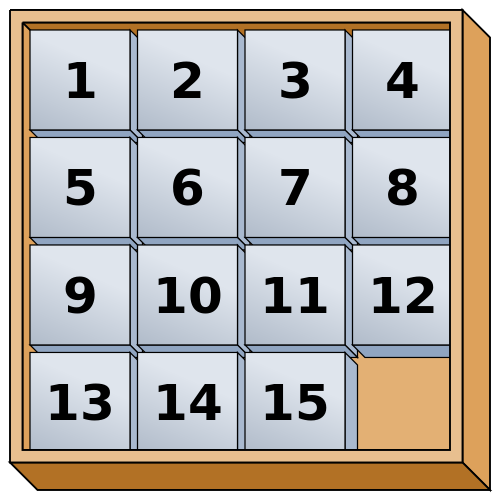
\includegraphics[width=1.5cm]{figs/15puzzle.png}};
      \node at (5,7) {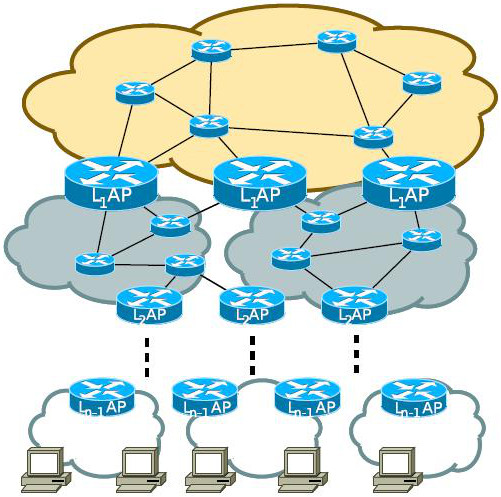
\includegraphics[width=1.5cm]{figs/internet-routers.jpg}};
      \node at (7,7) {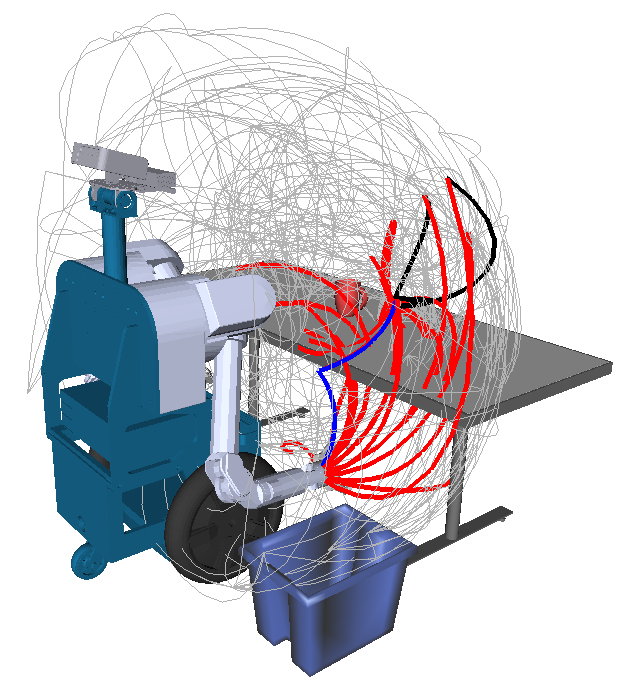
\includegraphics[width=1.5cm]{figs/lazysp-herbarm/herbarm-path33.png}};
      \node at (9,7) {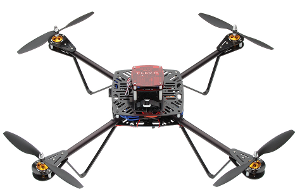
\includegraphics[width=1.5cm]{figs/quad.png}};
      \node at (11,7) {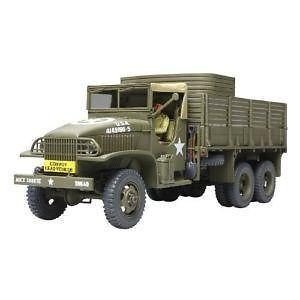
\includegraphics[width=1.5cm]{figs/military-truck.jpg}};
      
      % highlight nothing
      \only<1>{
         \fill[white,opacity=0.8] (0,6) rectangle (12,8);
      }
      
      % highlight puzzles
      \only<2-4>{
         \draw[ultra thick,rounded corners] (0.1,6.1) rectangle (3.9,7.9);
         \fill[white,opacity=0.8] (4,6) rectangle (12,8);
      }
      
      % highlight motion planning
      \only<5-10>{
         \draw[ultra thick,rounded corners] (6.1,6.1) rectangle (7.9,7.9);
         \fill[white,opacity=0.8] (0,6) rectangle (6,8);
         \fill[white,opacity=0.8] (8,6) rectangle (12,8);
         \only<6->{
            \node[align=center,font=\scriptsize] at (11.0,5.0) {Configuration\\Space};
         }
      }
      
      % highlight kinodynamic planning
      \only<11-12>{
         \draw[ultra thick,rounded corners] (8.1,6.1) rectangle (9.9,7.9);
         \fill[white,opacity=0.8] (0,6) rectangle (8,8);
         \fill[white,opacity=0.8] (10,6) rectangle (12,8);
         \node[align=center,font=\scriptsize] at (11.0,5.0) {Kinodynamic\\State Space};
      }
      
      % highlight convoy
      \only<13->{
         \draw[ultra thick,rounded corners] (10.1,6.1) rectangle (11.9,7.9);
         \fill[white,opacity=0.8] (0,6) rectangle (10,8);
         \only<15->{
            \node[draw,align=center,font=\scriptsize] (satnode) at (11.0,5.5) {Satellite};
         }
      }
      
      \node[draw,align=center,minimum height=1.0cm,minimum width=4cm,thick]
         (alg) at (6,0.55) {Shortest Path\\Algorithm};
      \draw[->] (4.5,1.40) -- (4.5,1.05);
      \draw[->] (7.5,1.40) -- (7.5,1.05);
      \node[draw,align=center,shape=document,minimum width=3.0cm,ultra thin]
         (query) at (2,0.55) {Query $v_s$, $v_t$\;\;};
      \draw[->] (query.east) -- (alg.west);
      \node[draw,align=center,shape=document,minimum width=2.0cm,ultra thin]
         (path) at (10,0.55) {Path $p^*$\;};
      \draw[->] (alg.east) -- (path.west);
   
   \end{tikzpicture}
\end{frame}

\begin{frame}
   \frametitle{Pathfinding with Expensive Edge Evaluations}
   
   In some domains, determining edge weights\\
   is a computationally expensive operation.
   
   \pause
   \vspace{0.4cm}
   \emph{Question: How can we solve shortest-path problems\\
      \quad \quad \quad \quad \, while reducing the number of edges evaluated?}
   
   \pause
   \vspace{0.4cm}
   Outline:
   \begin{itemize}
   \pause
   \item Review of lazy search approaches
   \pause
   \item LazySP algorithm outline (using \emph{edge selectors})
   \pause
   \item Equivalence to existing algorithms
   \pause
   \item Novel edge selectors
   %\pause
   %\item Experimental results
   \end{itemize}
\end{frame}

\begin{frame}
   \frametitle{Review of Prior Approaches}
   
   \begin{tikzpicture}[font=\small]
      \tikzset{>=latex} % arrow heads
      
      \draw[step=1,black!15,very thin,opacity=\gridopacity] (0,0) grid (12,8);
      
      % graph start
      \coordinate (va) at ( 2.0,5.6);
      \coordinate (vb) at ( 3.5,6.3);
      \coordinate (vc) at ( 4.0,7.5);
      \coordinate (vd) at ( 5.5,6.1);
      \coordinate (ve) at ( 8.0,6.6);
      \coordinate (vf) at (10.0,5.6);
      \coordinate (vg) at ( 1.5,6.6);
      \coordinate (vh) at ( 4.0,5.1);
      \coordinate (vi) at ( 7.0,4.8);
      \coordinate (vj) at ( 6.5,7.1);
      \coordinate (vk) at ( 9.0,5.1);
      
      % start/goal highlighting
      \node[circle,fill=black!20,inner sep=0.1cm] at (va) {};
      \node[circle,fill=black!20,inner sep=0.1cm] at (vf) {};
      
      % edges, grey
      \only<1-2,4,10>{
         \draw[black!30] (va) -- (vb) coordinate [midway] (eab);
         \draw[black!30] (vb) -- (vc) coordinate [midway] (ebc);
         \draw[black!30] (vb) -- (vd) coordinate [midway] (ebd);
         \draw[black!30] (vc) -- (vd) coordinate [midway] (ecd);
         \draw[black!30] (vd) -- (ve) coordinate [midway] (ede);
         \draw[black!30] (ve) -- (vf) coordinate [midway] (eef);
         \draw[black!30] (va) -- (vg) coordinate [midway] (eag);
         \draw[black!30] (vb) -- (vg) coordinate [midway] (ebg);
         \draw[black!30] (va) -- (vh) coordinate [midway] (eah);
         \draw[black!30] (vd) -- (vh) coordinate [midway] (edh);
         \draw[black!30] (vb) -- (vh) coordinate [midway] (ebh);
         \draw[black!30] (vd) -- (vi) coordinate [midway] (edi);
         \draw[black!30] (ve) -- (vi) coordinate [midway] (eei);
         \draw[black!30] (vc) -- (vj) coordinate [midway] (ecj);
         \draw[black!30] (vd) -- (vj) coordinate [midway] (edj);
         \draw[black!30] (ve) -- (vj) coordinate [midway] (eej);
         \draw[black!30] (vf) -- (vk) coordinate [midway] (efk);
         \draw[black!30] (vi) -- (vk) coordinate [midway] (eik);
         \draw[black!30] (ve) -- (vk) coordinate [midway] (eek);
         
         \node[circle,inner sep=0.02cm,fill=white,opacity=0.9,font=\scriptsize] at (eab) {?};
         \node[circle,inner sep=0.02cm,fill=white,opacity=0.9,font=\scriptsize] at (ebc) {?};
         \node[circle,inner sep=0.02cm,fill=white,opacity=0.9,font=\scriptsize] at (ebd) {?};
         \node[circle,inner sep=0.02cm,fill=white,opacity=0.9,font=\scriptsize] at (ecd) {?};
         \node[circle,inner sep=0.02cm,fill=white,opacity=0.9,font=\scriptsize] at (ede) {?};
         \node[circle,inner sep=0.02cm,fill=white,opacity=0.9,font=\scriptsize] at (eef) {?};
         \node[circle,inner sep=0.02cm,fill=white,opacity=0.9,font=\scriptsize] at (eag) {?};
         \node[circle,inner sep=0.02cm,fill=white,opacity=0.9,font=\scriptsize] at (ebg) {?};
         \node[circle,inner sep=0.02cm,fill=white,opacity=0.9,font=\scriptsize] at (eah) {?};
         \node[circle,inner sep=0.02cm,fill=white,opacity=0.9,font=\scriptsize] at (edh) {?};
         \node[circle,inner sep=0.02cm,fill=white,opacity=0.9,font=\scriptsize] at (ebh) {?};
         \node[circle,inner sep=0.02cm,fill=white,opacity=0.9,font=\scriptsize] at (edi) {?};
         \node[circle,inner sep=0.02cm,fill=white,opacity=0.9,font=\scriptsize] at (eei) {?};
         \node[circle,inner sep=0.02cm,fill=white,opacity=0.9,font=\scriptsize] at (ecj) {?};
         \node[circle,inner sep=0.02cm,fill=white,opacity=0.9,font=\scriptsize] at (edj) {?};
         \node[circle,inner sep=0.02cm,fill=white,opacity=0.9,font=\scriptsize] at (eej) {?};
         \node[circle,inner sep=0.02cm,fill=white,opacity=0.9,font=\scriptsize] at (efk) {?};
         \node[circle,inner sep=0.02cm,fill=white,opacity=0.9,font=\scriptsize] at (eik) {?};
         \node[circle,inner sep=0.02cm,fill=white,opacity=0.9,font=\scriptsize] at (eek) {?};
      }
      
      % edges, black
      \only<3>{
         \draw[ultra thick] (va) -- (vb) coordinate [midway] (eab);
         \draw[ultra thick] (vb) -- (vc) coordinate [midway] (ebc);
         \draw[ultra thick] (vb) -- (vd) coordinate [midway] (ebd);
         \draw[ultra thick] (vc) -- (vd) coordinate [midway] (ecd);
         \draw[ultra thick] (vd) -- (ve) coordinate [midway] (ede);
         \draw[ultra thick] (ve) -- (vf) coordinate [midway] (eef);
         \draw[ultra thick] (va) -- (vg) coordinate [midway] (eag);
         \draw[ultra thick] (vb) -- (vg) coordinate [midway] (ebg);
         \draw[ultra thick] (va) -- (vh) coordinate [midway] (eah);
         \draw[ultra thick] (vd) -- (vh) coordinate [midway] (edh);
         \draw[ultra thick] (vb) -- (vh) coordinate [midway] (ebh);
         \draw[ultra thick] (vd) -- (vi) coordinate [midway] (edi);
         \draw[ultra thick] (ve) -- (vi) coordinate [midway] (eei);
         \draw[ultra thick] (vc) -- (vj) coordinate [midway] (ecj);
         \draw[ultra thick] (vd) -- (vj) coordinate [midway] (edj);
         \draw[ultra thick] (ve) -- (vj) coordinate [midway] (eej);
         \draw[ultra thick] (vf) -- (vk) coordinate [midway] (efk);
         \draw[ultra thick] (vi) -- (vk) coordinate [midway] (eik);
         \draw[ultra thick] (ve) -- (vk) coordinate [midway] (eek);
         
         \node[circle,inner sep=0.02cm,fill=white,opacity=0.9,font=\scriptsize] at (eab) {5};
         \node[circle,inner sep=0.02cm,fill=white,opacity=0.9,font=\scriptsize] at (ebc) {5};
         \node[circle,inner sep=0.02cm,fill=white,opacity=0.9,font=\scriptsize] at (ebd) {6};
         \node[circle,inner sep=0.02cm,fill=white,opacity=0.9,font=\scriptsize] at (ecd) {7};
         \node[circle,inner sep=0.02cm,fill=white,opacity=0.9,font=\scriptsize] at (ede) {9};
         \node[circle,inner sep=0.02cm,fill=white,opacity=0.9,font=\scriptsize] at (eef) {7};
         \node[circle,inner sep=0.02cm,fill=white,opacity=0.9,font=\scriptsize] at (eag) {3};
         \node[circle,inner sep=0.02cm,fill=white,opacity=0.9,font=\scriptsize] at (ebg) {6};
         \node[circle,inner sep=0.02cm,fill=white,opacity=0.9,font=\scriptsize] at (eah) {6};
         \node[circle,inner sep=0.02cm,fill=white,opacity=0.9,font=\scriptsize] at (edh) {7};
         \node[circle,inner sep=0.02cm,fill=white,opacity=0.9,font=\scriptsize] at (ebh) {5};
         \node[circle,inner sep=0.02cm,fill=white,opacity=0.9,font=\scriptsize] at (edi) {8};
         \node[circle,inner sep=0.02cm,fill=white,opacity=0.9,font=\scriptsize] at (eei) {8};
         \node[circle,inner sep=0.02cm,fill=white,opacity=0.9,font=\scriptsize] at (ecj) {8};
         \node[circle,inner sep=0.02cm,fill=white,opacity=0.9,font=\scriptsize] at (edj) {6};
         \node[circle,inner sep=0.02cm,fill=white,opacity=0.9,font=\scriptsize] at (eej) {4};
         \node[circle,inner sep=0.02cm,fill=white,opacity=0.9,font=\scriptsize] at (efk) {3};
         \node[circle,inner sep=0.02cm,fill=white,opacity=0.9,font=\scriptsize] at (eik) {6};
         \node[circle,inner sep=0.02cm,fill=white,opacity=0.9,font=\scriptsize] at (eek) {6};
      }
      
      % NEXT, A* stuff
      
      % OPEN list highlighting (A*)
      \only<5>{\node[circle,fill=blue!70,inner sep=0.15cm] at (va) {};}
      \only<6-9>{\node[circle,fill=black!40,inner sep=0.15cm] at (va) {};}
      \only<6>{\node[circle,fill=blue!70,inner sep=0.15cm] at (vb) {};}
      \only<7-9>{\node[circle,fill=black!40,inner sep=0.15cm] at (vb) {};}
      \only<6-9>{\node[circle,fill=blue!40,inner sep=0.15cm] at (vg) {};}
      \only<6>{\node[circle,fill=blue!40,inner sep=0.15cm] at (vh) {};}
      \only<7>{\node[circle,fill=blue!70,inner sep=0.15cm] at (vh) {};}
      \only<8-9>{\node[circle,fill=black!40,inner sep=0.15cm] at (vh) {};}
      \only<7>{\node[circle,fill=blue!40,inner sep=0.15cm] at (vc) {};}
      \only<8>{\node[circle,fill=blue!70,inner sep=0.15cm] at (vc) {};}
      \only<9>{\node[circle,fill=black!40,inner sep=0.15cm] at (vc) {};}
      \only<7-9>{\node[circle,fill=blue!40,inner sep=0.15cm] at (vd) {};}
      \only<9>{\node[circle,fill=blue!70,inner sep=0.15cm] at (vj) {};}
      
      % first expansion
      \only<5>{
         \draw[black!30] (va) -- (vb) node[midway,circle,inner sep=0.02cm,fill=white,opacity=0.9,font=\scriptsize] {?};
         \draw[black!30] (va) -- (vg) node[midway,circle,inner sep=0.02cm,fill=white,opacity=0.9,font=\scriptsize] {?};
         \draw[black!30] (va) -- (vh) node[midway,circle,inner sep=0.02cm,fill=white,opacity=0.9,font=\scriptsize] {?};
      }
      \only<6-9>{
         \draw[black,ultra thick] (va) -- (vb) node[midway,circle,inner sep=0.02cm,fill=white,opacity=0.9,font=\scriptsize] {5};
         \draw[black,ultra thick] (va) -- (vg) node[midway,circle,inner sep=0.02cm,fill=white,opacity=0.9,font=\scriptsize] {3};
         \draw[black,ultra thick] (va) -- (vh) node[midway,circle,inner sep=0.02cm,fill=white,opacity=0.9,font=\scriptsize] {6};
      }
      % second expansion
      \only<5-6>{
         \draw[black!30] (vb) -- (vc) node[midway,circle,inner sep=0.02cm,fill=white,opacity=0.9,font=\scriptsize] {?};
         \draw[black!30] (vb) -- (vd) node[midway,circle,inner sep=0.02cm,fill=white,opacity=0.9,font=\scriptsize] {?};
         \draw[black!30] (vb) -- (vg) node[midway,circle,inner sep=0.02cm,fill=white,opacity=0.9,font=\scriptsize] {?};
         \draw[black!30] (vb) -- (vh) node[midway,circle,inner sep=0.02cm,fill=white,opacity=0.9,font=\scriptsize] {?};
      }
      \only<7-9>{
         \draw[black,ultra thick] (vb) -- (vc) node[midway,circle,inner sep=0.02cm,fill=white,opacity=0.9,font=\scriptsize] {5};
         \draw[black,ultra thick] (vb) -- (vd) node[midway,circle,inner sep=0.02cm,fill=white,opacity=0.9,font=\scriptsize] {$\infty$};
         \draw[black,ultra thick] (vb) -- (vg) node[midway,circle,inner sep=0.02cm,fill=white,opacity=0.9,font=\scriptsize] {6};
         \draw[black,ultra thick] (vb) -- (vh) node[midway,circle,inner sep=0.02cm,fill=white,opacity=0.9,font=\scriptsize] {5};
      }
      % third expansion
      \only<5-7>{
         \draw[black!30] (vd) -- (vh) node[midway,circle,inner sep=0.02cm,fill=white,opacity=0.9,font=\scriptsize] {?};
      }
      \only<8-9>{
         \draw[black,ultra thick] (vd) -- (vh) node[midway,circle,inner sep=0.02cm,fill=white,opacity=0.9,font=\scriptsize] {$\infty$};
      }
      % fourth expansion
      \only<5-8>{
         \draw[black!30] (vc) -- (vd) node[midway,circle,inner sep=0.02cm,fill=white,opacity=0.9,font=\scriptsize] {?};
         \draw[black!30] (vc) -- (vj) node[midway,circle,inner sep=0.02cm,fill=white,opacity=0.9,font=\scriptsize] {?};
      }
      \only<9>{
         \draw[black,ultra thick] (vc) -- (vd) node[midway,circle,inner sep=0.02cm,fill=white,opacity=0.9,font=\scriptsize] {$\infty$};
         \draw[black,ultra thick] (vc) -- (vj) node[midway,circle,inner sep=0.02cm,fill=white,opacity=0.9,font=\scriptsize] {8};
      }
      
      % edges, grey
      \only<5-9>{
         \draw[black!30] (vd) -- (ve) node[midway,circle,inner sep=0.02cm,fill=white,opacity=0.9,font=\scriptsize] {?};
         \draw[black!30] (ve) -- (vf) node[midway,circle,inner sep=0.02cm,fill=white,opacity=0.9,font=\scriptsize] {?};
         \draw[black!30] (vd) -- (vi) node[midway,circle,inner sep=0.02cm,fill=white,opacity=0.9,font=\scriptsize] {?};
         \draw[black!30] (ve) -- (vi) node[midway,circle,inner sep=0.02cm,fill=white,opacity=0.9,font=\scriptsize] {?};
         \draw[black!30] (vd) -- (vj) node[midway,circle,inner sep=0.02cm,fill=white,opacity=0.9,font=\scriptsize] {?};
         \draw[black!30] (ve) -- (vj) node[midway,circle,inner sep=0.02cm,fill=white,opacity=0.9,font=\scriptsize] {?};
         \draw[black!30] (vf) -- (vk) node[midway,circle,inner sep=0.02cm,fill=white,opacity=0.9,font=\scriptsize] {?};
         \draw[black!30] (vi) -- (vk) node[midway,circle,inner sep=0.02cm,fill=white,opacity=0.9,font=\scriptsize] {?};
         \draw[black!30] (ve) -- (vk) node[midway,circle,inner sep=0.02cm,fill=white,opacity=0.9,font=\scriptsize] {?};
      }
      
      % END A* stuff
      
      % NEXT, LWA* stuff
      
      % OPEN vertex list highlighting (LWA*)
      \only<11>{\node[circle,fill=blue!70,inner sep=0.15cm] at (va) {};}
      \only<12->{\node[circle,fill=black!40,inner sep=0.15cm] at (va) {};}
      \only<13>{\node[circle,fill=blue!70,inner sep=0.15cm] at (vb) {};}
      \only<14->{\node[circle,fill=black!40,inner sep=0.15cm] at (vb) {};}
      \only<15->{\node[circle,fill=blue!40,inner sep=0.15cm] at (vd) {};}
      \only<16>{\node[circle,fill=blue!70,inner sep=0.15cm] at (vh) {};}
      \only<17->{\node[circle,fill=black!40,inner sep=0.15cm] at (vh) {};}
      \only<19>{\node[circle,fill=blue!70,inner sep=0.15cm] at (vc) {};}
      \only<20->{\node[circle,fill=black!40,inner sep=0.15cm] at (vc) {};}
      \only<21>{\node[circle,fill=blue!70,inner sep=0.15cm] at (vj) {};}
      
      % edge queue
      \only<12->{\draw[blue!40,line width=0.10cm,line cap=round] (va) -- (vg);}
      \only<12-14>{\draw[blue!40,line width=0.10cm,line cap=round] (va) -- (vh);}
      \only<12>{\draw[blue!70,line width=0.10cm,line cap=round] (va) -- (vb);}
      \only<14-17>{\draw[blue!40,line width=0.10cm,line cap=round] (vb) -- (vc);}
      \only<14->{\draw[blue!40,line width=0.10cm,line cap=round] (vb) -- (vg);}
      \only<14->{\draw[blue!40,line width=0.10cm,line cap=round] (vb) -- (vh);}
      \only<14>{\draw[blue!70,line width=0.10cm,line cap=round] (vb) -- (vd);}
      \only<15>{\draw[blue!70,line width=0.10cm,line cap=round] (va) -- (vh);}
      \only<17>{\draw[blue!70,line width=0.10cm,line cap=round] (vh) -- (vd);}
      \only<18>{\draw[blue!70,line width=0.10cm,line cap=round] (vb) -- (vc);}
      \only<20->{\draw[blue!40,line width=0.10cm,line cap=round] (vc) -- (vd);}
      \only<20>{\draw[blue!70,line width=0.10cm,line cap=round] (vc) -- (vj);}
      
      \only<11-12>{
         \draw[black!30] (va) -- (vb) node[midway,circle,inner sep=0.02cm,fill=white,opacity=0.9,font=\scriptsize] {5?};
      }
      \only<13->{
         \draw[black,ultra thick] (va) -- (vb) node[midway,circle,inner sep=0.02cm,fill=white,opacity=0.9,font=\scriptsize] {5};
      }
      \only<11-14>{
         \draw[black!30] (vb) -- (vd) node[midway,circle,inner sep=0.02cm,fill=white,opacity=0.9,font=\scriptsize] {6?};
      }
      \only<15->{
         \draw[black,ultra thick] (vb) -- (vd) node[midway,circle,inner sep=0.02cm,fill=white,opacity=0.9,font=\scriptsize] {$\infty$};
      }
      \only<11-15>{
         \draw[black!30] (va) -- (vh) node[midway,circle,inner sep=0.02cm,fill=white,opacity=0.9,font=\scriptsize] {6?};
      }
      \only<16->{
         \draw[black,ultra thick] (va) -- (vh) node[midway,circle,inner sep=0.02cm,fill=white,opacity=0.9,font=\scriptsize] {6};
      }
      \only<11-17>{
         \draw[black!30] (vh) -- (vd) node[midway,circle,inner sep=0.02cm,fill=white,opacity=0.9,font=\scriptsize] {7?};
      }
      \only<18->{
         \draw[black,ultra thick] (vh) -- (vd) node[midway,circle,inner sep=0.02cm,fill=white,opacity=0.9,font=\scriptsize] {$\infty$};
      }
      \only<11-18>{
         \draw[black!30] (vb) -- (vc) node[midway,circle,inner sep=0.02cm,fill=white,opacity=0.9,font=\scriptsize] {5?};
      }
      \only<19->{
         \draw[black,ultra thick] (vb) -- (vc) node[midway,circle,inner sep=0.02cm,fill=white,opacity=0.9,font=\scriptsize] {5};
      }
      \only<11-20>{
         \draw[black!30] (vc) -- (vj) node[midway,circle,inner sep=0.02cm,fill=white,opacity=0.9,font=\scriptsize] {8?};
      }
      \only<21->{
         \draw[black,ultra thick] (vc) -- (vj) node[midway,circle,inner sep=0.02cm,fill=white,opacity=0.9,font=\scriptsize] {8};
      }
      
      % edges, grey
      \only<11->{
         \draw[black!30] (va) -- (vg) node[midway,circle,inner sep=0.02cm,fill=white,opacity=0.9,font=\scriptsize] {3?};
         \draw[black!30] (vb) -- (vg) node[midway,circle,inner sep=0.02cm,fill=white,opacity=0.9,font=\scriptsize] {6?};
         \draw[black!30] (vb) -- (vh) node[midway,circle,inner sep=0.02cm,fill=white,opacity=0.9,font=\scriptsize] {5?};
         \draw[black!30] (vc) -- (vd) node[midway,circle,inner sep=0.02cm,fill=white,opacity=0.9,font=\scriptsize] {7?};
         \draw[black!30] (vd) -- (ve) node[midway,circle,inner sep=0.02cm,fill=white,opacity=0.9,font=\scriptsize] {9?};
         \draw[black!30] (ve) -- (vf) node[midway,circle,inner sep=0.02cm,fill=white,opacity=0.9,font=\scriptsize] {7?};
         \draw[black!30] (vd) -- (vi) node[midway,circle,inner sep=0.02cm,fill=white,opacity=0.9,font=\scriptsize] {8?};
         \draw[black!30] (ve) -- (vi) node[midway,circle,inner sep=0.02cm,fill=white,opacity=0.9,font=\scriptsize] {8?};
         \draw[black!30] (vd) -- (vj) node[midway,circle,inner sep=0.02cm,fill=white,opacity=0.9,font=\scriptsize] {6?};
         \draw[black!30] (ve) -- (vj) node[midway,circle,inner sep=0.02cm,fill=white,opacity=0.9,font=\scriptsize] {4?};
         \draw[black!30] (vf) -- (vk) node[midway,circle,inner sep=0.02cm,fill=white,opacity=0.9,font=\scriptsize] {3?};
         \draw[black!30] (vi) -- (vk) node[midway,circle,inner sep=0.02cm,fill=white,opacity=0.9,font=\scriptsize] {6?};
         \draw[black!30] (ve) -- (vk) node[midway,circle,inner sep=0.02cm,fill=white,opacity=0.9,font=\scriptsize] {6?};
      }
      
      % END LWA* stuff
      
      \node[circle,fill=black,inner sep=0.05cm] at (va) {};
      \node[circle,fill=black,inner sep=0.05cm] at (vb) {};
      \node[circle,fill=black,inner sep=0.05cm] at (vc) {};
      \node[circle,fill=black,inner sep=0.05cm] at (vd) {};
      \node[circle,fill=black,inner sep=0.05cm] at (ve) {};
      \node[circle,fill=black,inner sep=0.05cm] at (vf) {};
      \node[circle,fill=black,inner sep=0.05cm] at (vg) {};
      \node[circle,fill=black,inner sep=0.05cm] at (vh) {};
      \node[circle,fill=black,inner sep=0.05cm] at (vi) {};
      \node[circle,fill=black,inner sep=0.05cm] at (vj) {};
      \node[circle,fill=black,inner sep=0.05cm] at (vk) {};

      \node[left=0.1cm of va] {$v_s$};
      \node[right=0.1cm of vf] {$v_t$};
      % graph end
      
      \only<2-3>{
         \node[fill=blue!20,anchor=north,rounded corners] at (6,4.4) {\begin{minipage}{11cm}
            \hangindent=0.35cm
            Approach 0: Pre-evaluate all edges, run SP algorithm.
         \end{minipage}};
      }
      \only<4->{
         \node[fill=blue!10,anchor=north,rounded corners] at (6,4.4) {\begin{minipage}{11cm}
            \hangindent=0.35cm
            Approach 0: Pre-evaluate all edges, run SP algorithm.
         \end{minipage}};
      }
      
      \only<4-9>{
         \node[fill=blue!20,anchor=north,rounded corners] at (6,3.57) {\begin{minipage}{11cm}
            \hangindent=0.35cm
            Approach 1: Run SP (e.g. A*) with JIT and memoized evaluations.\\
            (analogue to implicit graph representation)
         \end{minipage}};
      }
      \only<10->{
         \node[fill=blue!10,anchor=north,rounded corners] at (6,3.57) {\begin{minipage}{11cm}
            \hangindent=0.35cm
            Approach 1: Run SP (e.g. A*) with JIT and memoized evaluations.\\
            (analogue to implicit graph representation)
         \end{minipage}};
      }
      
      \only<10->{
         \node[fill=blue!20,anchor=north,rounded corners] at (6,2.3) {\begin{minipage}{11cm}
            \hangindent=0.35cm
            Approach 2: Lazy Weighted A* (LWA*). Uses weight estimator $w_{\ms{est}}$.\\
            Maintain independent vertex and edge queues.
         \end{minipage}};
      }
      
      \only<10->{
      %\begin{scope}
      %\clip (0,0) rectangle (12,8);
      \node[inner sep=0cm] at (6,0.55) {\begin{minipage}{11.0cm}\scriptsize
         
         \hangindent=0.35cm \raggedright
         \PaperPortrait\; Cohen, Phillips, and Likhachev,
         ``Planning Single-arm Manipulations with n-Arm Robots,''
         RSS 2014.
         
         \hangindent=0.35cm \raggedright
         \PaperPortrait\; Gammell, Srinivasa, and Barfoot,
         ``Batch Informed Trees (BIT*),''
         ICRA 2015.
      
      \end{minipage}};
      %\end{scope}
      }
      
   \end{tikzpicture}
   
\end{frame}

\begin{frame}
   \frametitle{Lazy Shortest Path: Best-First Search over Paths}
   \begin{tikzpicture}[font=\small]
      \draw[step=1,black!15,very thin,opacity=\gridopacity] (0,0) grid (12,8);
      
      % graph start
      \coordinate (va) at ( 2.0,5.6);
      \coordinate (vb) at ( 3.5,6.3);
      \coordinate (vc) at ( 4.0,7.5);
      \coordinate (vd) at ( 5.5,6.1);
      \coordinate (ve) at ( 8.0,6.6);
      \coordinate (vf) at (10.0,5.6);
      \coordinate (vg) at ( 1.5,6.6);
      \coordinate (vh) at ( 4.0,5.1);
      \coordinate (vi) at ( 7.0,4.8);
      \coordinate (vj) at ( 6.5,7.1);
      \coordinate (vk) at ( 9.0,5.1);
      
      % start/goal highlighting
      \node[circle,fill=black!20,inner sep=0.1cm] at (va) {};
      \node[circle,fill=black!20,inner sep=0.1cm] at (vf) {};
      
      % candidate paths
      \only<6-12>{
         \draw[line width=0.2cm,color=black!30,line cap=round]
            (va) -- (vb) -- (vd) -- (ve) -- (vf);
      }
      \only<9-11>{
         \draw[line width=0.2cm,color=blue!70,line cap=round]
            (vd) -- (ve);
      }
      \only<14-16>{
         \draw[line width=0.2cm,color=black!30,line cap=round]
            (va) -- (vb) -- (vd) -- (vj) -- (ve) -- (vf);
      }
      \only<15>{
         \draw[line width=0.2cm,color=blue!70,line cap=round]
            (vj) -- (ve);
      }
         
      \only<1-2>{
         \draw[black!30] (va) -- (vb);
         \draw[black!30] (vb) -- (vd);
         \draw[black!30] (va) -- (vh);
         \draw[black!30] (vh) -- (vd);
         \draw[black!30] (vb) -- (vc);
         \draw[black!30] (vc) -- (vj);
         \draw[black!30] (va) -- (vg);
         \draw[black!30] (vb) -- (vg);
         \draw[black!30] (vb) -- (vh);
         \draw[black!30] (vc) -- (vd);
         \draw[black!30] (vd) -- (ve);
         \draw[black!30] (ve) -- (vf);
         \draw[black!30] (vd) -- (vi);
         \draw[black!30] (ve) -- (vi);
         \draw[black!30] (vd) -- (vj);
         \draw[black!30] (ve) -- (vj);
         \draw[black!30] (vf) -- (vk);
         \draw[black!30] (vi) -- (vk);
         \draw[black!30] (ve) -- (vk);
      }
      \only<3->{
         \draw[black!30] (va) -- (vb) node[midway,circle,inner sep=0.02cm,fill=white,opacity=0.9,font=\scriptsize] {5?};
         \draw[black!30] (vb) -- (vd) node[midway,circle,inner sep=0.02cm,fill=white,opacity=0.9,font=\scriptsize] {6?};
         \draw[black!30] (va) -- (vh) node[midway,circle,inner sep=0.02cm,fill=white,opacity=0.9,font=\scriptsize] {6?};
         \draw[black!30] (vh) -- (vd) node[midway,circle,inner sep=0.02cm,fill=white,opacity=0.9,font=\scriptsize] {7?};
         \draw[black!30] (vb) -- (vc) node[midway,circle,inner sep=0.02cm,fill=white,opacity=0.9,font=\scriptsize] {5?};
         \draw[black!30] (vc) -- (vj) node[midway,circle,inner sep=0.02cm,fill=white,opacity=0.9,font=\scriptsize] {8?};
         \draw[black!30] (va) -- (vg) node[midway,circle,inner sep=0.02cm,fill=white,opacity=0.9,font=\scriptsize] {3?};
         \draw[black!30] (vb) -- (vg) node[midway,circle,inner sep=0.02cm,fill=white,opacity=0.9,font=\scriptsize] {6?};
         \draw[black!30] (vb) -- (vh) node[midway,circle,inner sep=0.02cm,fill=white,opacity=0.9,font=\scriptsize] {5?};
         \draw[black!30] (vc) -- (vd) node[midway,circle,inner sep=0.02cm,fill=white,opacity=0.9,font=\scriptsize] {7?};
         \draw[black!30] (ve) -- (vf) node[midway,circle,inner sep=0.02cm,fill=white,opacity=0.9,font=\scriptsize] {7?};
         \draw[black!30] (vd) -- (vi) node[midway,circle,inner sep=0.02cm,fill=white,opacity=0.9,font=\scriptsize] {8?};
         \draw[black!30] (ve) -- (vi) node[midway,circle,inner sep=0.02cm,fill=white,opacity=0.9,font=\scriptsize] {8?};
         \draw[black!30] (vd) -- (vj) node[midway,circle,inner sep=0.02cm,fill=white,opacity=0.9,font=\scriptsize] {6?};
         \draw[black!30] (vf) -- (vk) node[midway,circle,inner sep=0.02cm,fill=white,opacity=0.9,font=\scriptsize] {3?};
         \draw[black!30] (vi) -- (vk) node[midway,circle,inner sep=0.02cm,fill=white,opacity=0.9,font=\scriptsize] {6?};
         \draw[black!30] (ve) -- (vk) node[midway,circle,inner sep=0.02cm,fill=white,opacity=0.9,font=\scriptsize] {6?};
      }
      \only<3-11>{
         \draw[black!30] (vd) -- (ve) node[midway,circle,inner sep=0.02cm,fill=white,opacity=0.9,font=\scriptsize] {9?};
      }
      \only<12->{
         \draw[black,ultra thick] (vd) -- (ve) node[midway,circle,inner sep=0.02cm,fill=white,opacity=0.9,font=\scriptsize] {$\infty$};
      }
      \only<3-15>{
         \draw[black!30] (ve) -- (vj) node[midway,circle,inner sep=0.02cm,fill=white,opacity=0.9,font=\scriptsize] {4?};
      }
      \only<16->{
         \draw[black,ultra thick] (ve) -- (vj) node[midway,circle,inner sep=0.02cm,fill=white,opacity=0.9,font=\scriptsize] {4};
      }
      \node[circle,fill=black,inner sep=0.05cm] at (va) {};
      \node[circle,fill=black,inner sep=0.05cm] at (vb) {};
      \node[circle,fill=black,inner sep=0.05cm] at (vc) {};
      \node[circle,fill=black,inner sep=0.05cm] at (vd) {};
      \node[circle,fill=black,inner sep=0.05cm] at (ve) {};
      \node[circle,fill=black,inner sep=0.05cm] at (vf) {};
      \node[circle,fill=black,inner sep=0.05cm] at (vg) {};
      \node[circle,fill=black,inner sep=0.05cm] at (vh) {};
      \node[circle,fill=black,inner sep=0.05cm] at (vi) {};
      \node[circle,fill=black,inner sep=0.05cm] at (vj) {};
      \node[circle,fill=black,inner sep=0.05cm] at (vk) {};

      \node[left=0.1cm of va] {$v_s$};
      \node[right=0.1cm of vf] {$v_t$};
      % graph end
      
      % here's an algorithm
      
      \node[inner sep=0.2cm,fill=blue!10,rounded corners,anchor=north,minimum height=4.3cm,minimum width=7.5cm] (algbox) at (4.0,4.5) {};
      \node[inner sep=0.0cm,below=0.2cm of algbox.north,anchor=north]
      {\hspace*{-0.6cm}\begin{minipage}{7.5cm}\small{
      \algrenewcommand{\alglinenumber}[1]{}
      \begin{algorithmic}[1]
         \Function {\textsc{LazySP}}{$G, v_s, v_g, w, w_{\ms{est}}$}
         \only<3->{
            \State $E_{\ms{eval}} \leftarrow \emptyset$
            \State $w_{\ms{lazy}}(e) \leftarrow w_{\ms{est}}(e) \quad \forall e \in E$
         }
         \only<4->{
         \Loop
            \only<5->{
               \State $p_{\ms{candidate}} \leftarrow
                  \mbox{\sc InnerSP}(G, v_s, v_g, w_{\ms{lazy}})$ %\Comment Compute the shortest path with lazy edge weights
            }
            %\vspace{0.2cm}
            %\If {$p_{\ms{candidate}} \subseteq E_{\ms{eval}}$} \Comment If path is fully evaluated,
            %   \State \Return $p_{\ms{candidate}}$ \Comment return it
            %\EndIf
            \only<7->{
               \State \textbf{if} $p_{\ms{candidate}} \subseteq E_{\ms{eval}}$ \textbf{then return} $p_{\ms{candidate}}$
            }
            \only<8->{
               \vspace{0.1cm}
               \State $E_{\ms{selected}} \leftarrow  \mbox{\sc EdgeSelector}(G, p_{\ms{candidate}})$ %\Comment Select edges on path to process
            }
            \only<10->{
            \For {$e \in E_{\ms{selected}} \setminus E_{\ms{eval}}$} %\Comment For all unevaluated selected edges
               \only<11->{
                  \State $w_{\ms{lazy}}(e) \leftarrow w(e)$
                  \State $E_{\ms{eval}} \leftarrow E_{\ms{eval}} \cup e$ %\Comment Add to evaluated edge set
               }
            \EndFor
            }
         \EndLoop
         }
         \EndFunction
      \end{algorithmic}
      }\end{minipage}};

      \only<2-16>{
         \node[align=center,fill=black!5,rounded corners,minimum width=2.5cm] at (10.0,3.5)
         {\begin{minipage}{3.5cm}
            For motion planning,
            \vspace{-0.2cm}
            \[
               w(e) = \left\{ \arraycolsep=2pt \begin{array}{cl}
                  ||e|| & e \in C_{\ms{free}} \\
                  \infty & \mbox{otherwise}
                  \end{array} \right.
            \]
            \vspace{-0.4cm}
            \[
               w_{\ms{est}}(e) = ||e||
            \]
         \end{minipage}};
      }
      
      \only<18->{
         \node[align=center,fill=blue!10,rounded corners,minimum width=2.5cm] at (10.0,3.5)
            {\textbf{Complete}};
      }
      
      \only<19->{
         \node[align=center,fill=blue!10,rounded corners,minimum width=2.5cm] at (10.0,2)
            {\textbf{Optimal}\\(or bounded\\suboptimal)};
      }
      
   %Augment problem with inexpensive edge heuristic. (Show augmentation.)
   %Each edge has binary state.
   
   %Show outline of algorithm.
   
   %Two core sub-routines: inner SP search, and edge selector.
   \end{tikzpicture}
\end{frame}

%\fi

%\begin{frame}
%   \frametitle{Theoretical Properties of LazySP}
%   
%   \begin{tikzpicture}
%      \draw[step=1,black!15,very thin,opacity=\gridopacity] (0,0) grid (12,8);
%   
%      \node[inner sep=0.2cm,fill=blue!10,rounded corners] at (6,5) {\begin{minipage}{11cm}\small{
%         \textbf{Completeness.} If {\sc InnerSP} is complete,
%         {\sc EdgeSelector} always returns one unevaluated edge on
%         $p_{\ms{candidate}}$,
%         and $G$ is finite,
%         then {\sc LazySP} is complete.
%      }\end{minipage}};
%      
%      \node[inner sep=0.2cm,fill=blue!10,rounded corners] at (6,3) {\begin{minipage}{11cm}\small{
%         \textbf{Bounded suboptimality.}
%         If {\sc InnerSP} is optimal
%         and $w_{\ms{est}} \leq \epsilon \, w$
%         for some $\epsilon \geq 1$,
%         then the solution $p$ returned by {\sc LazySP}
%         satisfies $\mbox{len}(p) \leq \epsilon \, \ell^*$
%         with $\ell^*$ the length of an optimal path.
%      }\end{minipage}};
%   \end{tikzpicture}
%   
%\end{frame}

\begin{frame}
   \frametitle{Relation to the Dynamic Traversal Problem}
   \begin{tikzpicture}
      \draw[step=1,black!15,very thin,opacity=\gridopacity] (0,0) grid (12,8);
      
      \node at (1.7,6) {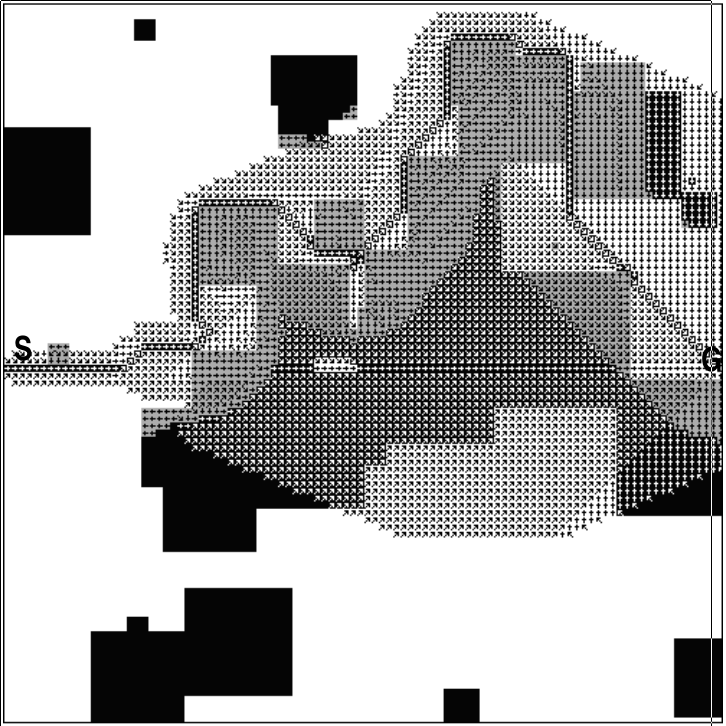
\includegraphics[width=3cm]{figs/dstar.png}};
      
      \node[anchor=north] at (7.6,7.6) {\begin{minipage}{9cm}
         \begin{itemize}
         \raggedright
         \item An agent conducting a traversal continually
         replans an optimal path in response to updated edge weights
         (e.g. via robot sensors).
         
         \only<2->{
         \item Algorithms: D*, Focussed D*, D* Lite.
         }
         
         \only<3->{
         \item Changed edges are treated as a property of the problem
         domain.
         }
         \end{itemize}
      \end{minipage}};
      
      \only<4->{
      \node[fill=blue!20,anchor=north,rounded corners] at (6,4.2)
      {\begin{minipage}{10cm}
         In contrast,
         the expensive-evaluation pathfinding problem allows for
         edges to be evaluated arbitrarily.
      \end{minipage}};
      }
      
      \only<5->{
      \node[fill=blue!20,anchor=north,rounded corners] at (6,2.9)
      {\begin{minipage}{10cm}
         LazySP exploits this freedom to focus its evaluations
         via appropriate choice of the edge selector.
      \end{minipage}};
      }
      
      \only<2->{
      \node[inner sep=0pt] at (6,0.8) {\begin{minipage}{11.5cm}\scriptsize{
         \hangindent=0.35cm \raggedright
         \PaperPortrait\; Stentz,
         ``Optimal and Efficient Path Planning for Partially-Known
         Environments,'' ICRA 1994.
         
         \hangindent=0.35cm \raggedright
         \PaperPortrait\; Stentz,
         ``The Focussed {D}* Algorithm for Real-Time Replanning,''
         IJCAI 1995.
         
         \hangindent=0.35cm \raggedright
         \PaperPortrait\; Koenig and Likhachev,
         ``D* Lite,'' AAAI 2002.
      }\end{minipage}};
      }
      
   \end{tikzpicture}
\end{frame}

\begin{frame}
   \frametitle{Simple Edge Selectors and Equivalences}
   \begin{tikzpicture}
      \draw[step=1,black!15,very thin,opacity=\gridopacity] (0,0) grid (12,8);
      \tikzset{>=latex}
   
   
      \only<2->{
      \node[fill=blue!20,anchor=north,rounded corners,
         minimum width=5.8cm,minimum height=3cm] (blockexp) at (3,7.8) {};
      \node[anchor=north,below=0cm of blockexp.north]
      {\begin{minipage}{5.5cm}
         \textbf{LazySP w/ Expand Selector}
         
         (all out-edges of frontier vertex)
      \end{minipage}};
      \begin{scope}[scale=0.5,shift={(1.75,10.2)}]
      
         \fill[white,opacity=0.7,rounded corners] (-1.3,-0.4) rectangle (9.8,3.2);
      
         % graph start
         \coordinate (va) at ( 0.5,0.8);
         \coordinate (vb) at ( 2.0,1.5);
         \coordinate (vc) at ( 2.5,2.7);
         \coordinate (vd) at ( 4.0,1.3);
         \coordinate (ve) at ( 6.5,1.8);
         \coordinate (vf) at ( 8.5,0.8);
         \coordinate (vg) at ( 0.0,1.8);
         \coordinate (vh) at ( 2.5,0.3);
         \coordinate (vi) at ( 5.5,0.0);
         \coordinate (vj) at ( 5.0,2.3);
         \coordinate (vk) at ( 7.5,0.3);
         
         % start/goal highlighting
         \node[circle,fill=black!20,inner sep=0.1cm] at (va) {};
         \node[circle,fill=black!20,inner sep=0.1cm] at (vf) {};
         
         \only<3->{
         % candidate path
         \draw[line width=0.2cm,color=black!30,line cap=round]
            (va) -- (vb) -- (vd) -- (ve) -- (vf);
         }
         
         \only<4->{
         % highlight first unevaled edge
         \draw[line width=0.4cm,color=blue!50!white,line cap=round] (vb) -- (vd);
         \draw[line width=0.2cm,color=black!30,line cap=round] (vb) -- (vd);
         }
         
         \only<5->{
         % point to frontier vertex
         \draw[blue!50!white,->,ultra thick] (0.5,3.0) -- (1.5,2.0);
         }
         
         % edges
         \draw[black,ultra thick] (va) -- (vb);
         \draw[black!30] (vb) -- (vd);
         \draw[black,ultra thick] (va) -- (vh);
         \draw[black!30] (vh) -- (vd);
         \draw[black!30] (vb) -- (vc);
         \draw[black!30] (vc) -- (vj);
         \draw[black,ultra thick] (va) -- (vg);
         \draw[black!30] (vb) -- (vg);
         \draw[black!30] (vb) -- (vh);
         \draw[black!30] (vc) -- (vd);
         \draw[black!30] (vd) -- (ve);
         \draw[black!30] (ve) -- (vf);
         \draw[black!30] (vd) -- (vi);
         \draw[black!30] (ve) -- (vi);
         \draw[black!30] (vd) -- (vj);
         \draw[black!30] (ve) -- (vj);
         \draw[black!30] (vf) -- (vk);
         \draw[black!30] (vi) -- (vk);
         \draw[black!30] (ve) -- (vk);
         
         \only<6->{
         % highlight edges to return
         \draw[blue,ultra thick] (va) -- (vb);
         \draw[blue,ultra thick] (vb) -- (vc);
         \draw[blue,ultra thick] (vb) -- (vd);
         \draw[blue,ultra thick] (vb) -- (vg);
         \draw[blue,ultra thick] (vb) -- (vh);
         }
         
         % nodes
         \node[circle,fill=black,inner sep=0.05cm] at (va) {};
         \node[circle,fill=black,inner sep=0.05cm] at (vb) {};
         \node[circle,fill=black,inner sep=0.05cm] at (vc) {};
         \node[circle,fill=black,inner sep=0.05cm] at (vd) {};
         \node[circle,fill=black,inner sep=0.05cm] at (ve) {};
         \node[circle,fill=black,inner sep=0.05cm] at (vf) {};
         \node[circle,fill=black,inner sep=0.05cm] at (vg) {};
         \node[circle,fill=black,inner sep=0.05cm] at (vh) {};
         \node[circle,fill=black,inner sep=0.05cm] at (vi) {};
         \node[circle,fill=black,inner sep=0.05cm] at (vj) {};
         \node[circle,fill=black,inner sep=0.05cm] at (vk) {};
      \end{scope}
      }
      \only<7->{
      \node[fill=blue!20,anchor=north,rounded corners,
         minimum width=5.8cm,minimum height=3cm] (blockexp) at (9,7.8) {};
      \node[anchor=north,below=0cm of blockexp.north]
      {\begin{minipage}{5.5cm}
         \textbf{Weighted A*}
         
         with JIT/memoized evaluations
         
      \end{minipage}};
      \node[anchor=south,above=0cm of blockexp.south]
      {\begin{minipage}{5.5cm}\scriptsize
      
         \hangindent=0.35cm \raggedright
         \PaperPortrait\; Pohl,
         ``Heuristic Search Viewed as Path Finding in a Graph,''
         AI 1970.
      
      \end{minipage}};
      \node[fill=white,opacity=0.9,inner sep=0.1cm,rounded corners] at (6,6.3) {\LARGE =};
      }
      
      
      
      \only<8->{
      \node[fill=blue!20,anchor=north,rounded corners,
         minimum width=5.8cm,minimum height=3cm] (blockfwd) at (3,4.5) {};
      \node[anchor=north,below=0cm of blockfwd.north]
      {\begin{minipage}{5.5cm}
         \textbf{LazySP w/ Forward Selector}
         
         (first unevaluated edge)
      \end{minipage}};
      \begin{scope}[scale=0.5,shift={(1.75,3.6)}]
      
         \fill[white,opacity=0.7,rounded corners] (-1.3,-0.4) rectangle (9.8,3.2);
      
         % graph start
         \coordinate (va) at ( 0.5,0.8);
         \coordinate (vb) at ( 2.0,1.5);
         \coordinate (vc) at ( 2.5,2.7);
         \coordinate (vd) at ( 4.0,1.3);
         \coordinate (ve) at ( 6.5,1.8);
         \coordinate (vf) at ( 8.5,0.8);
         \coordinate (vg) at ( 0.0,1.8);
         \coordinate (vh) at ( 2.5,0.3);
         \coordinate (vi) at ( 5.5,0.0);
         \coordinate (vj) at ( 5.0,2.3);
         \coordinate (vk) at ( 7.5,0.3);
         
         % start/goal highlighting
         \node[circle,fill=black!20,inner sep=0.1cm] at (va) {};
         \node[circle,fill=black!20,inner sep=0.1cm] at (vf) {};
         
         \only<9->{
         % candidate path
         \draw[line width=0.2cm,color=black!30,line cap=round]
            (va) -- (vb) -- (vd) -- (ve) -- (vf);
         }
         
         \only<10->{
         % highlight first unevaled edge
         \draw[line width=0.4cm,color=blue!50!white,line cap=round] (vb) -- (vd);
         \draw[line width=0.2cm,color=black!30,line cap=round] (vb) -- (vd);
         }
         
         % edges
         \draw[black,ultra thick] (va) -- (vb);
         \draw[black!30] (vb) -- (vd);
         \draw[black,ultra thick] (va) -- (vh);
         \draw[black!30] (vh) -- (vd);
         \draw[black!30] (vb) -- (vc);
         \draw[black!30] (vc) -- (vj);
         \draw[black,ultra thick] (va) -- (vg);
         \draw[black!30] (vb) -- (vg);
         \draw[black!30] (vb) -- (vh);
         \draw[black!30] (vc) -- (vd);
         \draw[black!30] (vd) -- (ve);
         \draw[black!30] (ve) -- (vf);
         \draw[black!30] (vd) -- (vi);
         \draw[black!30] (ve) -- (vi);
         \draw[black!30] (vd) -- (vj);
         \draw[black!30] (ve) -- (vj);
         \draw[black!30] (vf) -- (vk);
         \draw[black!30] (vi) -- (vk);
         \draw[black!30] (ve) -- (vk);
         
         \only<10->{
         % highlight edges to return
         \draw[blue,ultra thick] (vb) -- (vd);
         }
         
         % nodes
         \node[circle,fill=black,inner sep=0.05cm] at (va) {};
         \node[circle,fill=black,inner sep=0.05cm] at (vb) {};
         \node[circle,fill=black,inner sep=0.05cm] at (vc) {};
         \node[circle,fill=black,inner sep=0.05cm] at (vd) {};
         \node[circle,fill=black,inner sep=0.05cm] at (ve) {};
         \node[circle,fill=black,inner sep=0.05cm] at (vf) {};
         \node[circle,fill=black,inner sep=0.05cm] at (vg) {};
         \node[circle,fill=black,inner sep=0.05cm] at (vh) {};
         \node[circle,fill=black,inner sep=0.05cm] at (vi) {};
         \node[circle,fill=black,inner sep=0.05cm] at (vj) {};
         \node[circle,fill=black,inner sep=0.05cm] at (vk) {};
      \end{scope}
      }
      
      \only<11->{
      \node[fill=blue!20,anchor=north,rounded corners,
         minimum width=5.8cm,minimum height=3cm] (blockexp) at (9,4.5) {};
      \node[anchor=north,below=0cm of blockexp.north]
      {\begin{minipage}{5.5cm}
         \textbf{Lazy Weighted A*}
         
         with JIT/memoized evaluations
         
      \end{minipage}};
      \node[anchor=south,above=0cm of blockexp.south]
      {\begin{minipage}{5.5cm}\scriptsize
      
         \hangindent=0.35cm 
         \PaperPortrait\; Cohen, Phillips, and Likhachev,
         ``Planning Single-arm Manipulations with n-Arm Robots,''
         RSS 2014.
      
      \end{minipage}};
      \node[fill=white,opacity=0.9,inner sep=0.1cm,rounded corners] at (6,3.0) {\LARGE =};
      }
      
      \only<7->{
      \node[fill=black!20,rounded corners] at (6,0.75)
      {\begin{minipage}{7.3cm}
         Edge-equivalence: algorithms will evaluate
         the same edges in the same order.
      \end{minipage}};
      }
   
   \end{tikzpicture}
\end{frame}

\begin{frame}
   \frametitle{Other Simple Edge Selectors}
   \begin{tikzpicture}
      \draw[step=1,black!15,very thin,opacity=\gridopacity] (0,0) grid (12,8);
      \tikzset{>=latex}
      
      
      
      \node[fill=blue!20,anchor=north,rounded corners,
         minimum width=5.8cm,minimum height=3cm] (blockexp) at (3,7.8) {};
      \node[anchor=north,below=0cm of blockexp.north]
      {\begin{minipage}{5.5cm}
         \textbf{LazySP w/ Forward Selector}
         
         (first unevaluated edge)
      \end{minipage}};
      \begin{scope}[scale=0.5,shift={(1.75,10.2)}]
      
         \fill[white,opacity=0.7,rounded corners] (-1.3,-0.4) rectangle (9.8,3.2);
      
         % graph start
         \coordinate (va) at ( 0.5,0.8);
         \coordinate (vb) at ( 2.0,1.5);
         \coordinate (vc) at ( 2.5,2.7);
         \coordinate (vd) at ( 4.0,1.3);
         \coordinate (ve) at ( 6.5,1.8);
         \coordinate (vf) at ( 8.5,0.8);
         \coordinate (vg) at ( 0.0,1.8);
         \coordinate (vh) at ( 2.5,0.3);
         \coordinate (vi) at ( 5.5,0.0);
         \coordinate (vj) at ( 5.0,2.3);
         \coordinate (vk) at ( 7.5,0.3);
         
         % start/goal highlighting
         \node[circle,fill=black!20,inner sep=0.1cm] at (va) {};
         \node[circle,fill=black!20,inner sep=0.1cm] at (vf) {};
         
         % candidate path
         \draw[line width=0.2cm,color=black!30,line cap=round]
            (va) -- (vb) -- (vd) -- (ve) -- (vf);
         
         % highlight first unevaled edge
         \draw[line width=0.4cm,color=blue!50!white,line cap=round] (vb) -- (vd);
         \draw[line width=0.2cm,color=black!30,line cap=round] (vb) -- (vd);
         
         % edges
         \draw[black,ultra thick] (va) -- (vb);
         \draw[black!30] (vb) -- (vd);
         \draw[black,ultra thick] (va) -- (vh);
         \draw[black!30] (vh) -- (vd);
         \draw[black!30] (vb) -- (vc);
         \draw[black!30] (vc) -- (vj);
         \draw[black,ultra thick] (va) -- (vg);
         \draw[black!30] (vb) -- (vg);
         \draw[black!30] (vb) -- (vh);
         \draw[black!30] (vc) -- (vd);
         \draw[black!30] (vd) -- (ve);
         \draw[black!30] (ve) -- (vf);
         \draw[black!30] (vd) -- (vi);
         \draw[black!30] (ve) -- (vi);
         \draw[black!30] (vd) -- (vj);
         \draw[black!30] (ve) -- (vj);
         \draw[black!30] (vf) -- (vk);
         \draw[black!30] (vi) -- (vk);
         \draw[black!30] (ve) -- (vk);
         
         \draw[blue,ultra thick] (vb) -- (vd);
         
         % nodes
         \node[circle,fill=black,inner sep=0.05cm] at (va) {};
         \node[circle,fill=black,inner sep=0.05cm] at (vb) {};
         \node[circle,fill=black,inner sep=0.05cm] at (vc) {};
         \node[circle,fill=black,inner sep=0.05cm] at (vd) {};
         \node[circle,fill=black,inner sep=0.05cm] at (ve) {};
         \node[circle,fill=black,inner sep=0.05cm] at (vf) {};
         \node[circle,fill=black,inner sep=0.05cm] at (vg) {};
         \node[circle,fill=black,inner sep=0.05cm] at (vh) {};
         \node[circle,fill=black,inner sep=0.05cm] at (vi) {};
         \node[circle,fill=black,inner sep=0.05cm] at (vj) {};
         \node[circle,fill=black,inner sep=0.05cm] at (vk) {};
      \end{scope}
      
      
      
      \only<2->{
      \node[fill=blue!20,anchor=north,rounded corners,
         minimum width=5.8cm,minimum height=3cm] (blockexp) at (9,7.8) {};
      \node[anchor=north,below=0cm of blockexp.north]
      {\begin{minipage}{5.5cm}
         \textbf{LazySP w/ Reverse Selector}
         
         (last unevaluated edge)
      \end{minipage}};
      \begin{scope}[scale=0.5,shift={(13.75,10.2)}]
      
         \fill[white,opacity=0.7,rounded corners] (-1.3,-0.4) rectangle (9.8,3.2);
      
         % graph start
         \coordinate (va) at ( 0.5,0.8);
         \coordinate (vb) at ( 2.0,1.5);
         \coordinate (vc) at ( 2.5,2.7);
         \coordinate (vd) at ( 4.0,1.3);
         \coordinate (ve) at ( 6.5,1.8);
         \coordinate (vf) at ( 8.5,0.8);
         \coordinate (vg) at ( 0.0,1.8);
         \coordinate (vh) at ( 2.5,0.3);
         \coordinate (vi) at ( 5.5,0.0);
         \coordinate (vj) at ( 5.0,2.3);
         \coordinate (vk) at ( 7.5,0.3);
         
         % start/goal highlighting
         \node[circle,fill=black!20,inner sep=0.1cm] at (va) {};
         \node[circle,fill=black!20,inner sep=0.1cm] at (vf) {};
         
         % candidate path
         \draw[line width=0.2cm,color=black!30,line cap=round]
            (va) -- (vb) -- (vd) -- (ve) -- (vf);
         
         % highlight first unevaled edge
         \draw[line width=0.4cm,color=blue!50!white,line cap=round] (ve) -- (vf);
         \draw[line width=0.2cm,color=black!30,line cap=round] (ve) -- (vf);
         
         % edges
         \draw[black,ultra thick] (va) -- (vb);
         \draw[black!30] (vb) -- (vd);
         \draw[black,ultra thick] (va) -- (vh);
         \draw[black!30] (vh) -- (vd);
         \draw[black!30] (vb) -- (vc);
         \draw[black!30] (vc) -- (vj);
         \draw[black,ultra thick] (va) -- (vg);
         \draw[black!30] (vb) -- (vg);
         \draw[black!30] (vb) -- (vh);
         \draw[black!30] (vc) -- (vd);
         \draw[black!30] (vd) -- (ve);
         \draw[black!30] (ve) -- (vf);
         \draw[black!30] (vd) -- (vi);
         \draw[black!30] (ve) -- (vi);
         \draw[black!30] (vd) -- (vj);
         \draw[black!30] (ve) -- (vj);
         \draw[black!30] (vf) -- (vk);
         \draw[black!30] (vi) -- (vk);
         \draw[black!30] (ve) -- (vk);
         
         \draw[blue,ultra thick] (ve) -- (vf);
         
         % nodes
         \node[circle,fill=black,inner sep=0.05cm] at (va) {};
         \node[circle,fill=black,inner sep=0.05cm] at (vb) {};
         \node[circle,fill=black,inner sep=0.05cm] at (vc) {};
         \node[circle,fill=black,inner sep=0.05cm] at (vd) {};
         \node[circle,fill=black,inner sep=0.05cm] at (ve) {};
         \node[circle,fill=black,inner sep=0.05cm] at (vf) {};
         \node[circle,fill=black,inner sep=0.05cm] at (vg) {};
         \node[circle,fill=black,inner sep=0.05cm] at (vh) {};
         \node[circle,fill=black,inner sep=0.05cm] at (vi) {};
         \node[circle,fill=black,inner sep=0.05cm] at (vj) {};
         \node[circle,fill=black,inner sep=0.05cm] at (vk) {};
      \end{scope}
      }
      
      
      
      \only<3->{
      \node[fill=blue!20,anchor=north,rounded corners,
         minimum width=5.8cm,minimum height=3cm] (blockfwd) at (3,4.5) {};
      \node[anchor=north,below=0cm of blockfwd.north]
      {\begin{minipage}{5.5cm}
         \textbf{LazySP w/ Alternate Selector}
         
         (alternate Forward and Reverse)
      \end{minipage}};
      \begin{scope}[scale=0.5,shift={(1.75,3.6)}]
      
         \fill[white,opacity=0.7,rounded corners] (-1.3,-0.4) rectangle (9.8,3.2);
      
         % graph start
         \coordinate (va) at ( 0.5,0.8);
         \coordinate (vb) at ( 2.0,1.5);
         \coordinate (vc) at ( 2.5,2.7);
         \coordinate (vd) at ( 4.0,1.3);
         \coordinate (ve) at ( 6.5,1.8);
         \coordinate (vf) at ( 8.5,0.8);
         \coordinate (vg) at ( 0.0,1.8);
         \coordinate (vh) at ( 2.5,0.3);
         \coordinate (vi) at ( 5.5,0.0);
         \coordinate (vj) at ( 5.0,2.3);
         \coordinate (vk) at ( 7.5,0.3);
         
         % start/goal highlighting
         \node[circle,fill=black!20,inner sep=0.1cm] at (va) {};
         \node[circle,fill=black!20,inner sep=0.1cm] at (vf) {};
         
         % candidate path
         \draw[line width=0.2cm,color=black!30,line cap=round]
            (va) -- (vb) -- (vd) -- (ve) -- (vf);
         
         \only<4>{
         % highlight first unevaled edge
         \draw[line width=0.4cm,color=blue!50!white,line cap=round] (vb) -- (vd);
         \draw[line width=0.2cm,color=black!30,line cap=round] (vb) -- (vd);
         }
         \only<5>{
         % highlight first unevaled edge
         \draw[line width=0.4cm,color=blue!50!white,line cap=round] (ve) -- (vf);
         \draw[line width=0.2cm,color=black!30,line cap=round] (ve) -- (vf);
         }
         \only<6->{
         % highlight first unevaled edge
         \draw[line width=0.4cm,color=blue!50!white,line cap=round] (vd) -- (ve);
         \draw[line width=0.2cm,color=black!30,line cap=round] (vd) -- (ve);
         }
         
         % edges
         \draw[black,ultra thick] (va) -- (vb);
         \draw[black!30] (vb) -- (vd);
         \draw[black,ultra thick] (va) -- (vh);
         \draw[black!30] (vh) -- (vd);
         \draw[black!30] (vb) -- (vc);
         \draw[black!30] (vc) -- (vj);
         \draw[black,ultra thick] (va) -- (vg);
         \draw[black!30] (vb) -- (vg);
         \draw[black!30] (vb) -- (vh);
         \draw[black!30] (vc) -- (vd);
         \draw[black!30] (vd) -- (ve);
         \draw[black!30] (ve) -- (vf);
         \draw[black!30] (vd) -- (vi);
         \draw[black!30] (ve) -- (vi);
         \draw[black!30] (vd) -- (vj);
         \draw[black!30] (ve) -- (vj);
         \draw[black!30] (vf) -- (vk);
         \draw[black!30] (vi) -- (vk);
         \draw[black!30] (ve) -- (vk);
         
         % highlight edges to return
         \only<4>{\draw[blue,ultra thick] (vb) -- (vd);}
         \only<5->{\draw[black,ultra thick] (vb) -- (vd);}
         \only<5>{\draw[blue,ultra thick] (ve) -- (vf);}
         \only<6->{\draw[black,ultra thick] (ve) -- (vf);}
         \only<6->{\draw[blue,ultra thick] (vd) -- (ve);}
         
         % nodes
         \node[circle,fill=black,inner sep=0.05cm] at (va) {};
         \node[circle,fill=black,inner sep=0.05cm] at (vb) {};
         \node[circle,fill=black,inner sep=0.05cm] at (vc) {};
         \node[circle,fill=black,inner sep=0.05cm] at (vd) {};
         \node[circle,fill=black,inner sep=0.05cm] at (ve) {};
         \node[circle,fill=black,inner sep=0.05cm] at (vf) {};
         \node[circle,fill=black,inner sep=0.05cm] at (vg) {};
         \node[circle,fill=black,inner sep=0.05cm] at (vh) {};
         \node[circle,fill=black,inner sep=0.05cm] at (vi) {};
         \node[circle,fill=black,inner sep=0.05cm] at (vj) {};
         \node[circle,fill=black,inner sep=0.05cm] at (vk) {};
      \end{scope}
      }
      
      
      
      \only<7->{
      \node[fill=blue!20,anchor=north,rounded corners,
         minimum width=5.8cm,minimum height=3cm] (blockfwd) at (9,4.5) {};
      \node[anchor=north,below=0cm of blockfwd.north]
      {\begin{minipage}{5.5cm}
         \textbf{LazySP w/ Bisect Selector}
         
         (alternate Forward and Reverse)
      \end{minipage}};
      \begin{scope}[scale=0.5,shift={(13.75,3.6)}]
      
         \fill[white,opacity=0.7,rounded corners] (-1.3,-0.4) rectangle (9.8,3.2);
      
         % graph start
         \coordinate (va) at ( 0.5,0.8);
         \coordinate (vb) at ( 2.0,1.5);
         \coordinate (vc) at ( 2.5,2.7);
         \coordinate (vd) at ( 4.0,1.3);
         \coordinate (ve) at ( 6.5,1.8);
         \coordinate (vf) at ( 8.5,0.8);
         \coordinate (vg) at ( 0.0,1.8);
         \coordinate (vh) at ( 2.5,0.3);
         \coordinate (vi) at ( 5.5,0.0);
         \coordinate (vj) at ( 5.0,2.3);
         \coordinate (vk) at ( 7.5,0.3);
         
         % start/goal highlighting
         \node[circle,fill=black!20,inner sep=0.1cm] at (va) {};
         \node[circle,fill=black!20,inner sep=0.1cm] at (vf) {};
         
         % candidate path
         \draw[line width=0.2cm,color=black!30,line cap=round]
            (va) -- (vb) -- (vd) -- (ve) -- (vf);
         
         % highlight first unevaled edge
         \draw[line width=0.4cm,color=blue!50!white,line cap=round] (vd) -- (ve);
         \draw[line width=0.2cm,color=black!30,line cap=round] (vd) -- (ve);
         
         % edges
         \draw[black,ultra thick] (va) -- (vb);
         \draw[black!30] (vb) -- (vd);
         \draw[black,ultra thick] (va) -- (vh);
         \draw[black!30] (vh) -- (vd);
         \draw[black!30] (vb) -- (vc);
         \draw[black!30] (vc) -- (vj);
         \draw[black,ultra thick] (va) -- (vg);
         \draw[black!30] (vb) -- (vg);
         \draw[black!30] (vb) -- (vh);
         \draw[black!30] (vc) -- (vd);
         \draw[black!30] (vd) -- (ve);
         \draw[black!30] (ve) -- (vf);
         \draw[black!30] (vd) -- (vi);
         \draw[black!30] (ve) -- (vi);
         \draw[black!30] (vd) -- (vj);
         \draw[black!30] (ve) -- (vj);
         \draw[black!30] (vf) -- (vk);
         \draw[black!30] (vi) -- (vk);
         \draw[black!30] (ve) -- (vk);
         
         % highlight edges to return
         \draw[black,ultra thick] (vd) -- (ve);
         
         % nodes
         \node[circle,fill=black,inner sep=0.05cm] at (va) {};
         \node[circle,fill=black,inner sep=0.05cm] at (vb) {};
         \node[circle,fill=black,inner sep=0.05cm] at (vc) {};
         \node[circle,fill=black,inner sep=0.05cm] at (vd) {};
         \node[circle,fill=black,inner sep=0.05cm] at (ve) {};
         \node[circle,fill=black,inner sep=0.05cm] at (vf) {};
         \node[circle,fill=black,inner sep=0.05cm] at (vg) {};
         \node[circle,fill=black,inner sep=0.05cm] at (vh) {};
         \node[circle,fill=black,inner sep=0.05cm] at (vi) {};
         \node[circle,fill=black,inner sep=0.05cm] at (vj) {};
         \node[circle,fill=black,inner sep=0.05cm] at (vk) {};
      \end{scope}
      }
      
   
   \end{tikzpicture}
\end{frame}

\begin{frame}
   \frametitle{Novel Selectors: Path Distribution}
   
   \begin{center}
   \begin{tikzpicture}
      \draw[step=1,black!15,very thin,opacity=\gridopacity] (-6,-1.7) grid (6,1.7);
      \tikzset{>=latex}
      
      \only<2->{
         \node[draw,minimum width=2.4cm,minimum height=3.0cm] (startbox) at (-3.0,0) {};
         \node[inner sep=0pt] at (-3.0,-0.35) {\includegraphics[scale=2.0]{build/lazysp-fig-dists/fig-sofar}};
         \node[align=center,font=\footnotesize,below] at (startbox.north) {known\\edges};
      }
      
      \only<3->{
         \node[draw] (quesbox) at (-1.2,0) {?};
         \draw[->] (startbox) -- (quesbox);
      
         \node[draw,minimum width=2.1cm,minimum height=3.0cm] (pathsbox) at (0.4,0) {};
         \node[inner sep=0pt] at (-0.05, 0.1) {\includegraphics[scale=0.8]{build/lazysp-fig-dists/fig-path-00}};
         \node[inner sep=0pt] at ( 0.85, 0.1) {\includegraphics[scale=0.8]{build/lazysp-fig-dists/fig-path-01}};
         \node[inner sep=0pt] at (-0.05,-0.8) {\includegraphics[scale=0.8]{build/lazysp-fig-dists/fig-path-02}};
         \node[inner sep=0pt] at ( 0.85,-0.8) {\includegraphics[scale=0.8]{build/lazysp-fig-dists/fig-path-03}};
         \node[align=center,font=\footnotesize,below] at (pathsbox.north) {path\\distribution};
         \node[align=center,font=\normalsize,above] at (pathsbox.south) {$\dots$};
         \draw[->] (quesbox) -- (pathsbox);
      }
      
      \only<4->{
         \node[draw,minimum width=2.4cm,minimum height=3.0cm] (goalbox) at (3.0,0) {};
         \node[inner sep=0pt] at (3.0,-0.35) {\includegraphics[scale=2.0]{build/lazysp-fig-dists/fig-dist-probs}};
         \node[align=center,font=\footnotesize,below] at (goalbox.north) {edge indicator\\distributions};
         \draw[->] (pathsbox) -- (goalbox);
      }
   \end{tikzpicture}
   \end{center}
   
   Central idea behind novel selectors:
   \pause
   \begin{itemize}
   \item Given known edges and the current lazy edge weights,
   \pause
   \item propose some distribution $\mathcal{D}_p$ over potential paths,
   \pause
   \item and select the unevaluated edge that is
   \textbf{most likely} on the path drawn from $\mathcal{D}_p$.
   \end{itemize}
   
\end{frame}

\begin{frame}
   \frametitle{Path Distribution via Weight Function Sampling}
   \begin{tikzpicture}
      \draw[step=1,black!15,very thin,opacity=\gridopacity] (-7,-3.1) grid (5,4.9);
      \tikzset{>=latex}
      
      \node at (-1,4) {\begin{minipage}{11.0cm}
      \raggedright
      Given a distribution $\mathcal{D}_w$
      over consistent edge weight functions,
      compute the shortest path for each to form $\mathcal{D}_p$.
      \end{minipage}};
      
      \node[draw,minimum width=1.8cm,minimum height=2.6cm] (startbox) at (-4.4,0) {};
      \node[inner sep=0pt] at (-4.4,-0.35) {\includegraphics[scale=1.5]{build/lazysp-fig-dists/fig-sofar}};
      \node[align=center,font=\footnotesize,below] at (startbox.north) {known\\edges};
      
      \only<2->{
         \node[draw,minimum width=1.8cm,minimum height=6cm] (abox) at (-2.2,0) {};
         \node[inner sep=0pt] at (-2.2, 1.3) {\includegraphics[scale=1.5]{build/lazysp-fig-dists/fig-world-00}};
         \node[inner sep=0pt] at (-2.2,-0.3) {\includegraphics[scale=1.5]{build/lazysp-fig-dists/fig-world-01}};
         \node[inner sep=0pt] at (-2.2,-1.9) {\includegraphics[scale=1.5]{build/lazysp-fig-dists/fig-world-02}};
         \node[align=center,font=\footnotesize,below] at (abox.north) {obstacle\\distribution};
         \node[align=center,font=\normalsize,above] at (abox.south) {$\dots$};
         \draw[->] (startbox) -- (abox);
      }
      
      \only<3->{
         \node[draw,minimum width=1.8cm,minimum height=6cm] (bbox) at (0,0) {};
         \node[inner sep=0pt] at (0, 1.3) {\includegraphics[scale=1.5]{build/lazysp-fig-dists/fig-wfn-00}};
         \node[inner sep=0pt] at (0,-0.3) {\includegraphics[scale=1.5]{build/lazysp-fig-dists/fig-wfn-01}};
         \node[inner sep=0pt] at (0,-1.9) {\includegraphics[scale=1.5]{build/lazysp-fig-dists/fig-wfn-02}};
         \node[align=center,font=\footnotesize,below] at (bbox.north) {weight fn\\distribution};
         \node[align=center,font=\normalsize,above] at (bbox.south) {$\dots$};
         \draw[->] (abox) -- (bbox);
      }
      
      \only<4->{
         \node[draw,minimum width=1.8cm,minimum height=6cm] (cbox) at (2.2,0) {};
         \node[inner sep=0pt] at (2.2, 1.3) {\includegraphics[scale=1.5]{build/lazysp-fig-dists/fig-path-00}};
         \node[inner sep=0pt] at (2.2,-0.3) {\includegraphics[scale=1.5]{build/lazysp-fig-dists/fig-path-01}};
         \node[inner sep=0pt] at (2.2,-1.9) {\includegraphics[scale=1.5]{build/lazysp-fig-dists/fig-path-02}};
         \node[align=center,font=\footnotesize,below] at (cbox.north) {path\\distribution};
         \node[align=center,font=\normalsize,above] at (cbox.south) {$\dots$};
         \draw[->] (bbox) -- (cbox);
      }
      
   \end{tikzpicture}
\end{frame}

\begin{frame}
   \frametitle{Path Distribution via the Partition Function}
   
   \begin{itemize}
   \item
   Sampling weight functions and solving the corresponding SP problems
   can be expensive.
   
   \pause
   \item
   How else can we efficiently generate a reasonable distribution
   over potential paths?
   \end{itemize}
   
   \pause
   \begin{equation*}
      P: \mbox{set of all paths from $v_s$ to $v_t$}
   \end{equation*}%
   \pause%
   \vspace{-0.3cm}
   \begin{equation*}
      \arraycolsep=1pt
      \begin{array}{ll}
      \mathcal{D}_p : & \mbox{path distribution with PDF } \\
      & f(p) \propto \exp( - \beta \, \mbox{len}(p, w_{\ms{lazy}}) ). \\
      \end{array}
   \end{equation*}
   
   \pause
   \vspace{0.3cm}
   \begin{itemize}
   \item At each iteration,
   the shortest path in $P$
   (which is chosen as the LazySP candidate path)
   is most likely under $\mathcal{D}_p$ ...
   
   \pause
   \item ... but other paths also have probability mass,
      with longer paths exponentially less likely.
   \end{itemize}
   
\end{frame}

\begin{frame}
   \frametitle{Path Distribution via the Partition Function}
   \begin{tikzpicture}
      \draw[step=1,black!15,very thin,opacity=\gridopacity] (0,0) grid (12,8);
      \tikzset{>=latex}
   
      \node at (6,7.5) {
         Examples of the edge probabilities for various values of $\beta$:
      };
      
      \only<2->{
      \node (empty50) at (3,5.5) {\includegraphics{build/lazysp-selscores/empty-50}};
      \node[anchor=north west, below right=0.2cm of empty50.north west,font=\small] {$\beta=50$};
      }
      \only<3->{
      \node (empty33) at (6,5.5) {\includegraphics{build/lazysp-selscores/empty-33}};
      \node[anchor=north west, below right=0.2cm of empty33.north west,font=\small] {$\beta=33$};
      }
      \only<4->{
      \node (empty28) at (9,5.5) {\includegraphics{build/lazysp-selscores/empty-28}};
      \node[anchor=north west, below right=0.2cm of empty28.north west,font=\small] {$\beta=28$};
      }
      
      \only<5->{
      \node (gap50) at (3,2.3) {\includegraphics{build/lazysp-selscores/gap-50}};
      \node[anchor=north west, below right=0.2cm of gap50.north west,font=\small] {$\beta=50$};
      }
      \only<6->{
      \node (gap33) at (6,2.3) {\includegraphics{build/lazysp-selscores/gap-33}};
      \node[anchor=north west, below right=0.2cm of gap33.north west,font=\small] {$\beta=33$};
      }
      \only<7->{
      \node (gap28) at (9,2.3) {\includegraphics{build/lazysp-selscores/gap-28}};
      \node[anchor=north west, below right=0.2cm of gap28.north west,font=\small] {$\beta=28$};
      }
   
   \end{tikzpicture}
\end{frame}

\begin{frame}
   \frametitle{Partition Function: Incremental Formulation}
   
   Efficient implementation of the partition function selector
   requires an incremental algorithm for calculating $Z_{st}$ over $G$.
   
   \begin{equation*}
      P_{xy}: \mbox{set of all paths from $v_x$ to $v_y$}
   \end{equation*}
   \begin{equation*}
      Z_{xy} = \sum_{p \in P_{xy}} \exp( - \beta \, \mbox{len}(p) )
   \end{equation*}
   
   \pause
   Consider two directed graphs, $G=(V,E)$ and $G'=(V,E')$,
   with $E' = E \cup \{ e'_{ab} \}$
   and $z'_{ab} = \exp(-\beta w(e'_{ab}))$.
   Suppose that the values $Z_{xy}$ are known for all pairs $x,y$.
   Then we can write:
   \pause
   \begin{equation*}
      \arraycolsep=1pt
      \def\arraystretch{1.8}
      \begin{array}{ll}
      Z'_{xy}
         & = \left[ Z_{xy} \right]
         + \left[ Z_{xa} \, z'_{ab} \, Z_{by} \right]
         + \left[ Z_{xa} \, z'_{ab} \, Z_{ba} \, z'_{ab} \, Z_{by} \right]
         + \dots \\
      \pause
      & = Z_{xy} + \frac{\displaystyle Z_{xa} Z_{by}}{\displaystyle 1 / z'_{ab} - Z_{ba}}
      \end{array}
   \end{equation*}
   
\end{frame}

%\begin{frame}
%   \frametitle{Illustration of Selectors}
%   \begin{tikzpicture}
%      \draw[step=1,black!15,very thin,opacity=\gridopacity] (0,0) grid (12,8);
%      \tikzset{>=latex}
%      
%      \node at (0.9,7.0) {\footnotesize \strut Expand};
%      \node at (0.9,5.9) {\includegraphics[width=1.6cm]{build/lazysp-example-1/alg-fwdexpand-after5}};
%      \node at (0.9,4.1) {\includegraphics[width=1.6cm]{build/lazysp-example-1/alg-fwdexpand-end}};
%      \node at (0.9,2.5) {\includegraphics[width=1.6cm]{build/lazysp-example-1/alg-fwdexpand-path-bars}};
%   
%      \node at (2.6,7.0) {\footnotesize \strut Forward};
%      \node at (2.6,5.9) {\includegraphics[width=1.6cm]{build/lazysp-example-1/alg-fwd-after5}};
%      \node at (2.6,4.1) {\includegraphics[width=1.6cm]{build/lazysp-example-1/alg-fwd-end}};
%      \node at (2.6,2.5) {\includegraphics[width=1.6cm]{build/lazysp-example-1/alg-fwd-path-bars}};
%   
%      \node at (4.3,7.0) {\footnotesize \strut Reverse};
%      \node at (4.3,5.9) {\includegraphics[width=1.6cm]{build/lazysp-example-1/alg-rev-after5}};
%      \node at (4.3,4.1) {\includegraphics[width=1.6cm]{build/lazysp-example-1/alg-rev-end}};
%      \node at (4.3,2.5) {\includegraphics[width=1.6cm]{build/lazysp-example-1/alg-rev-path-bars}};
%   
%      \node at (6.0,7.0) {\footnotesize \strut Alternate};
%      \node at (6.0,5.9) {\includegraphics[width=1.6cm]{build/lazysp-example-1/alg-alt-after5}};
%      \node at (6.0,4.1) {\includegraphics[width=1.6cm]{build/lazysp-example-1/alg-alt-end}};
%      \node at (6.0,2.5) {\includegraphics[width=1.6cm]{build/lazysp-example-1/alg-alt-path-bars}};
%      
%      \node at (7.7,7.0) {\footnotesize \strut Bisect};
%      \node at (7.7,5.9) {\includegraphics[width=1.6cm]{build/lazysp-example-1/alg-bisect-after5}};
%      \node at (7.7,4.1) {\includegraphics[width=1.6cm]{build/lazysp-example-1/alg-bisect-end}};
%      \node at (7.7,2.5) {\includegraphics[width=1.6cm]{build/lazysp-example-1/alg-bisect-path-bars}};
%   
%      \node at (9.4,7.0) {\footnotesize \strut WeightSamp};
%      \node at (9.4,5.9) {\includegraphics[width=1.6cm]{build/lazysp-example-1/alg-worlddist1000-after5}};
%      \node at (9.4,4.1) {\includegraphics[width=1.6cm]{build/lazysp-example-1/alg-worlddist1000-end}};
%      \node at (9.4,2.5) {\includegraphics[width=1.6cm]{build/lazysp-example-1/alg-worlddist1000-path-bars}};
%   
%      \node at (11.1,7.0) {\footnotesize \strut Partition};
%      \node at (11.1,5.9) {\includegraphics[width=1.6cm]{build/lazysp-example-1/alg-partall-after5}};
%      \node at (11.1,4.1) {\includegraphics[width=1.6cm]{build/lazysp-example-1/alg-partall-end}};
%      \node at (11.1,2.5) {\includegraphics[width=1.6cm]{build/lazysp-example-1/alg-partall-path-bars}};
%   
%   \end{tikzpicture}
%\end{frame}

\begin{frame}
   \frametitle{Illustration of Selectors}
   \begin{tikzpicture}[font=\small]
      \draw[step=1,black!15,very thin,opacity=\gridopacity] (0,0) grid (12,8);
      \tikzset{>=latex}

      \begin{scope}[font=\footnotesize]
      \fill[blue] (0.2,6.9) circle (0.05cm);
      \fill[green] (0.4,6.9) circle (0.05cm);
      \node[anchor=west] at (0.6,6.9) {$q_s, q_t$};

      \draw[black!30,thick] (0.1,6.6) -- (0.5,6.6);
      \node[anchor=west] at (0.6,6.6) {$e$ unevaled};
      
      \draw[thick,black] (0.1,6.3) -- (0.5,6.3);
      \node[anchor=west] at (0.6,6.3) {$e \notin \mathcal{C}_{\ms{free}}$};
      
      \draw[thick,red] (0.1,6.0) -- (0.5,6.0);
      \node[anchor=west] at (0.6,6.0) {$e \in \mathcal{C}_{\ms{free}}$};
      \end{scope}

      \begin{scope}[font=\scriptsize]
      \node[anchor=west,align=center,inner sep=0pt] at (0.05,2.45) {for each unique path,\\the edges that are:};

      \draw[fill=black!10] (0.1,1.3) rectangle (0.3,2.1);
      \draw[fill=red!60!black] (0.1,1.1) rectangle (0.3,1.3);
      \draw[fill=green!60!black] (0.1,0.7) rectangle (0.3,1.1);
      \draw[fill=green!30!white] (0.1,0.1) rectangle (0.3,0.7);

      \node[anchor=west] at (0.45,1.7) {not evaled};
      \node[anchor=west] at (0.45,1.2) {evaled $\notin \mathcal{C}_{\ms{free}}$};
      \node[anchor=west] at (0.45,0.9) {evaled $\in \mathcal{C}_{\ms{free}}$};
      \node[anchor=west] at (0.45,0.4) {already evaled};

      \draw (0.2,1.7) -- (0.4,1.7);
      \draw (0.2,1.2) -- (0.4,1.2);
      \draw (0.2,0.9) -- (0.4,0.9);
      \draw (0.2,0.4) -- (0.4,0.4);
      \end{scope}

      \node[font=\scriptsize,black!50,rotate={90}] at (2.3,4.6) {$\downarrow$ Final \; 5 Edges $\downarrow$};
      
      %\node at (0.9,7.0) {\footnotesize \strut Expand};
      %\node at (0.9,5.9) {\includegraphics[width=1.6cm]{build/lazysp-example-1/alg-fwdexpand-after5}};
      %\node at (0.9,4.1) {\includegraphics[width=1.6cm]{build/lazysp-example-1/alg-fwdexpand-end}};
      %\node at (0.9,2.5) {\includegraphics[width=1.6cm]{build/lazysp-example-1/alg-fwdexpand-path-bars}};
   
      \node at (3.6,7.4) {\footnotesize \strut Forward};
      \node at (3.6,6.0) {\includegraphics[width=2.1cm]{build/lazysp-example-1/alg-fwd-after5}};
      \node at (3.6,3.5) {\includegraphics[width=2.1cm]{build/lazysp-example-1/alg-fwd-end}};
      \node at (3.6,1.2) {\includegraphics[width=2.1cm]{build/lazysp-example-1/alg-fwd-path-bars}};
   
      %\node at (4.3,7.0) {\footnotesize \strut Reverse};
      %\node at (4.3,5.9) {\includegraphics[width=1.6cm]{build/lazysp-example-1/alg-rev-after5}};
      %\node at (4.3,4.1) {\includegraphics[width=1.6cm]{build/lazysp-example-1/alg-rev-end}};
      %\node at (4.3,2.5) {\includegraphics[width=1.6cm]{build/lazysp-example-1/alg-rev-path-bars}};
   
      \node at (6.0,7.4) {\footnotesize \strut Alternate};
      \node at (6.0,6.0) {\includegraphics[width=2.1cm]{build/lazysp-example-1/alg-alt-after5}};
      \node at (6.0,3.5) {\includegraphics[width=2.1cm]{build/lazysp-example-1/alg-alt-end}};
      \node at (6.0,1.2) {\includegraphics[width=2.1cm]{build/lazysp-example-1/alg-alt-path-bars}};
      
      \node at (8.4,7.4) {\footnotesize \strut Bisect};
      \node at (8.4,6.0) {\includegraphics[width=2.1cm]{build/lazysp-example-1/alg-bisect-after5}};
      \node at (8.4,3.5) {\includegraphics[width=2.1cm]{build/lazysp-example-1/alg-bisect-end}};
      \node at (8.4,1.2) {\includegraphics[width=2.1cm]{build/lazysp-example-1/alg-bisect-path-bars}};

      %\node at (9.4,7.0) {\footnotesize \strut WeightSamp};
      %\node at (9.4,5.9) {\includegraphics[width=1.6cm]{build/lazysp-example-1/alg-worlddist1000-after5}};
      %\node at (9.4,4.1) {\includegraphics[width=1.6cm]{build/lazysp-example-1/alg-worlddist1000-end}};
      %\node at (9.4,2.5) {\includegraphics[width=1.6cm]{build/lazysp-example-1/alg-worlddist1000-path-bars}};
   
      \node at (10.8,7.4) {\footnotesize \strut Partition};
      \node at (10.8,6.0) {\includegraphics[width=2.1cm]{build/lazysp-example-1/alg-partall-after5}};
      \node at (10.8,3.5) {\includegraphics[width=2.1cm]{build/lazysp-example-1/alg-partall-end}};
      \node at (10.8,1.2) {\includegraphics[width=2.1cm]{build/lazysp-example-1/alg-partall-path-bars}};

   \end{tikzpicture}
\end{frame}

%\fi % for iffalse

%\begin{frame}
%   \frametitle{Experimental Results}
%   \begin{tikzpicture}
%      \draw[step=1,black!15,very thin,opacity=\gridopacity] (0,0) grid (12,8);
%      \tikzset{>=latex}
%   
%      \node at (6,7.25) {\begin{minipage}{11cm}
%         Problem domains:
%      \end{minipage}};
%      
%      \only<2->{
%      \node at (3.0,5.1) {\includegraphics{build/lazysp-partconn}};
%      \node at (3.0,6.3) {\footnotesize \textbf{PartConn}};
%      }
%      
%      \only<3->{
%      \node at (6.0,5.1) {\includegraphics[width=2.0cm]{build/lazysp-example-1/alg-partall-end}};
%      \node at (6.0,6.3) {\footnotesize \textbf{UnitSquare}};
%      }
%   
%      \only<4->{
%      \node at (9.0,5.1) {\includegraphics[width=2.0cm]{figs/lazysp-herbarm/herbarm-path33.png}};
%      \node at (9.0,6.3) {\footnotesize \textbf{ArmPlan}};
%      }
%   
%      \only<5->{
%      \node[anchor=north] at (6,3.5) {\begin{minipage}{11cm}
%   
%         Metrics:
%         \begin{itemize}
%         \item Primary metric: mean number of edge evaluations.
%         \only<6->{
%         \item Secondary metric: mean computation time.
%         }
%         \end{itemize}
%      
%      \end{minipage}};
%      }
%      
%      \only<6->{
%      \node[inner sep=0pt] at (6,0.4) {\begin{minipage}{11.5cm}\scriptsize{
%         \hangindent=0.35cm \raggedright
%         \PaperPortrait\; Extended version on arXiv with full timing results:
%         {\texttt http://arxiv.org/abs/1603.03490}
%      }\end{minipage}};
%      }
%   
%   \end{tikzpicture}
%\end{frame}

%\begin{frame}
%   \frametitle{Experiment: Robot Arm Motion Planning}
%   
%   \includegraphics[width=2.5cm]{figs/lazysp-herbarm/herbarm-roadmap.png}
%   \includegraphics[width=2.5cm]{figs/lazysp-herbarm/herbarm-path02.png}
%   \includegraphics[width=2.5cm]{figs/lazysp-herbarm/herbarm-path33.png}
%   \includegraphics[width=2.5cm]{figs/lazysp-herbarm/herbarm-path42.png}
%   \includegraphics[width=2.5cm]{figs/lazysp-herbarm/herbarm-path46.png}
%      
%\end{frame}

% to generate these:
% $ for a in fwdexpand fwd rev alt even bisect worlddist1000 partall; do echo -n "$a "; for p in prob-*; do grep eval_edge $p/alg-$a-log.txt | wc -l; done | python -c 'import sys; import math; l=map(float,sys.stdin.read().split()); avg=sum(l)/len(l); finstddev_corrected =  math.sqrt(sum([(val-avg)**2 for val in l])/(len(l)-1)); print avg, 1.96*finstddev_corrected / math.sqrt(len(l))'; done

\pgfplotstableread{
selector mean error
Expand 87.10 2.39
Forward 35.86 1.04
Reverse 34.84 1.04
Alternate 22.23 0.60
Bisect 44.81 1.11
WeightSamp 20.66 0.57
Partition 20.39 0.56
}{\datapartconn}

% NEW: (stderrmean)
%fwdexpand 87.099 2.38650510278
%fwd 35.858 1.03906664632
%rev 34.842 1.03572378546
%alt 22.227 0.597811717725
%even 22.409 0.622905876301
%bisect 44.809 1.10686298369
%worlddist1000 20.663 0.570900480258
%partall 20.395 0.564433840729


\pgfplotstableread{
selector mean error
Expand 69.21 2.55
Forward 27.29 1.03
Reverse 27.69 1.02
Alternate 17.82 0.60
Bisect 32.62 0.72
WeightSamp 15.58 0.47
Partition 14.08 0.46
}{\dataunitsquare}

% NEW: 1.96
%fwdexpand 69.2077777778 2.55028628499
%fwd 27.2888888889 1.02504835213
%rev 27.6922222222 1.02028477535
%alt 17.8211111111 0.597332883603
%even 14.6466666667 0.628278955306
%bisect 32.6233333333 0.721817175333
%worlddist1000 15.5766666667 0.473857034803
%partall 14.0833333333 0.455891208479


\pgfplotstableread{
selector mean error
Expand 115 0.01
Forward 63.62 4.15
Reverse 74.94 5.07
Alternate 55.48 2.95
Bisect 68.01 3.86
WeightSamp 56.93 3.37
Partition 48.07 2.44
}{\dataarmplan}

\pgfplotstableread{
selector mean error
Expand 115 0.01
Forward 63.62 4.15
Reverse 74.94 5.07
Alternate 0 0
Bisect 68.01 3.86
WeightSamp 56.93 3.37
Partition 48.07 2.44
}{\dataarmplannoalt}

\pgfplotstableread{
selector mean error
Expand 0 0
Forward 0 0
Reverse 0 0
Alternate 55.48 2.95
Bisect 0 0
WeightSamp 0 0
Partition 0 0
}{\dataarmplanonlyalt}

% NEW stderr
%Expand 949.0466666666664 63.46454650463161
%Forward 63.62000000000001 4.1478023030971745
%Reverse 74.93999999999998 5.070126727608847
%Alternate 55.47999999999999 2.950293578535276
%Even 63.99333333333334 3.994684563504954
%Bisect 68.01333333333332 3.86218318531321
%WeightSamp 60.99333333333333 3.651837545718 %% DIFFERENT!
%Partition 48.06666666666667 2.44118108287056


\begin{frame}
   \frametitle{Experimental Results: Edges Evaluated}
   \begin{tikzpicture}
      \draw[step=1,black!15,very thin,opacity=\gridopacity] (0,0) grid (12,8);
      \clip (0,0) rectangle (12,8);
      \tikzset{>=latex}
   
      \only<2->{
      \node at (2.1,7.8) {\footnotesize \textbf{PartConn}};
      \node at (2.1,6.6) {\includegraphics{build/lazysp-partconn}};
   
      \begin{scope}[shift={(5.5,5.5)}]
      \begin{axis}[
         width=7.0cm,
         height=4.0cm,
         xbar,
         bar width=7,
         xmin=0,xmax=95,
         %xtick pos=bottom,
         %symbolic y coords={E, F, R, A, B, W, P},
         yticklabels from table={\datapartconn}{selector},
         ytick=data,
         ytick pos=left,
         xmajorgrids,
         xmajorticks=false,
         ticklabel style={font=\footnotesize}
         ] 
      \node[circle,fill=white,inner sep=1pt,text=black!40] at (axis cs:40,-5.6) {\scriptsize 40};
      \node[circle,fill=white,inner sep=1pt,text=black!40] at (axis cs:60,-5.6) {\scriptsize 60};
      \node[circle,fill=white,inner sep=1pt,text=black!40] at (axis cs:80,-5.6) {\scriptsize 80};
      \addplot[color=black,fill=black!20,error bars/.cd,x dir=both,x explicit]
         table[y expr=-\coordindex,x=mean,x error expr=1.96*\thisrow{error}]
         {\datapartconn};
      \end{axis}
      \end{scope}
      }
      
      
      \only<3->{
      \node at (2.1,3.9) {\includegraphics[width=2.0cm]{build/lazysp-example-1/alg-partall-end}};
      \node at (2.1,5.1) {\footnotesize \textbf{UnitSquare}};
      
      \begin{scope}[shift={(5.5,2.8)}]
      \begin{axis}[
         width=7.0cm,
         height=4.0cm,
         xbar,
         bar width=7,
         xmin=0,xmax=95,
         %xtick pos=bottom,
         %symbolic y coords={E, F, R, A, B, W, P},
         yticklabels from table={\dataunitsquare}{selector},
         ytick=data,
         ytick pos=left,
         xmajorgrids,
         xmajorticks=false,
         ticklabel style={font=\footnotesize}
         ]
      \node[circle,fill=white,inner sep=1pt,text=black!40] at (axis cs:40,-5.6) {\scriptsize 40};
      \node[circle,fill=white,inner sep=1pt,text=black!40] at (axis cs:60,-5.6) {\scriptsize 60};
      \node[circle,fill=white,inner sep=1pt,text=black!40] at (axis cs:80,-5.6) {\scriptsize 80};
      \addplot[color=black,fill=black!20,error bars/.cd,x dir=both,x explicit]
         table[y expr=-\coordindex,x=mean,x error expr=1.96*\thisrow{error}]
         {\dataunitsquare};
      \end{axis}
      \end{scope}
      }
      
      
      \only<4->{
      \node at (2.1,1.15) {\includegraphics[width=2.0cm]{figs/lazysp-herbarm/herbarm-path33.png}};
      \node at (2.1,2.4) {\footnotesize \textbf{ArmPlan}};
      
      \begin{scope}[shift={(5.5,0.1)}]
      \begin{axis}[
         width=7.0cm,
         height=4.0cm,
         xbar stacked,
         bar width=7,
         xmin=0,xmax=115,
         %xtick pos=bottom,
         %symbolic y coords={E, F, R, A, B, W, P},
         yticklabels from table={\dataarmplan}{selector},
         ytick=data,
         ytick pos=left,
         xmajorgrids,
         xmajorticks=false,
         ticklabel style={font=\footnotesize}
         ]
      \node[circle,fill=white,inner sep=1pt,text=black!40] at (axis cs:60,-5.6) {\scriptsize 60};
      \node[circle,fill=white,inner sep=1pt,text=black!40] at (axis cs:80,-5.6) {\scriptsize 80};
      \node[circle,fill=white,inner sep=1pt,text=black!40] at (axis cs:100,-5.6) {\scriptsize 100};
      \only<4>{
         \addplot[color=black,fill=black!20,error bars/.cd,x dir=both,x explicit]
            table[y expr=-\coordindex,x=mean,x error expr=1.96*\thisrow{error}]
            {\dataarmplan};
      }
      \only<5>{
         \addplot[color=black,fill=black!20,error bars/.cd,x dir=both,x explicit]
            table[y expr=-\coordindex,x=mean,x error expr=1.96*\thisrow{error}]
            {\dataarmplannoalt};
         \addplot[color=black,fill=blue!40,error bars/.cd,x dir=both,x explicit]
            table[y expr=-\coordindex,x=mean,x error expr=1.96*\thisrow{error}]
            {\dataarmplanonlyalt};
      }
      \node[align=center,anchor=east,inner sep=0pt] at (axis cs:113,-0.05) {\scriptsize 949 $\rightarrow$};
      \end{axis}
      \end{scope}
      }
      
   \end{tikzpicture}
\end{frame}

\pgfplotstableread{
selector dursearch dursel dureval duronline-error
Expand      0.02  0.00 10.00 0.0001
Forward     0.02  0.00  5.87 0.46
Reverse     0.02  0.00  8.20 0.53
Alternate   0.02  0.00  5.94 0.31
Bisect      0.02  0.00  7.31 0.43
WeightSamp  0.02 10.00  9.39 0.0001
Partition   0.04  1.54  4.21 0.28
}{\dataarmplantime}

%\begin{frame}
%   \frametitle{Experimental Results: ArmPlan Computation Time}
%
%   \includegraphics[width=2.5cm]{figs/lazysp-herbarm/herbarm-roadmap.png}
%   \includegraphics[width=2.5cm]{figs/lazysp-herbarm/herbarm-path02.png}
%   \includegraphics[width=2.5cm]{figs/lazysp-herbarm/herbarm-path33.png}
%   \includegraphics[width=2.5cm]{figs/lazysp-herbarm/herbarm-path42.png}
%   \includegraphics[width=2.5cm]{figs/lazysp-herbarm/herbarm-path46.png}
%   
%   \begin{tikzpicture}
%      %\draw[step=1,black!15,very thin,opacity=\gridopacity] (0,0) grid (12,8);
%      \tikzset{>=latex}
%   
%      \begin{axis}[
%         width=7.0cm,
%         height=4.0cm,
%         xbar stacked,
%         bar width=7,
%         xmin=0,xmax=10,
%         %xtick pos=bottom,
%         %symbolic y coords={E, F, R, A, B, W, P},
%         yticklabels from table={\dataarmplantime}{selector},
%         ytick=data,
%         ytick pos=left,
%         xmajorgrids,
%         xmajorticks=false,
%         ticklabel style={font=\footnotesize}
%         ] 
%      \node[circle,fill=white,inner sep=1pt,text=black!40] at (axis cs:40,-5.6) {\scriptsize 40};
%      \node[circle,fill=white,inner sep=1pt,text=black!40] at (axis cs:60,-5.6) {\scriptsize 60};
%      \node[circle,fill=white,inner sep=1pt,text=black!40] at (axis cs:80,-5.6) {\scriptsize 80};
%      \addplot[color=black,fill=blue!30]
%         table[y expr=-\coordindex,x=dursearch]
%         {\dataarmplantime};
%      \addplot[color=black,fill=purple!20]
%         table[y expr=-\coordindex,x=dursel]
%         {\dataarmplantime};
%      \addplot[color=black,fill=green!20,error bars/.cd,x dir=both,x explicit]
%         table[y expr=-\coordindex,x=dureval,x error expr=\thisrow{duronline-error}]
%         {\dataarmplantime};
%      \end{axis}
%      
%   \end{tikzpicture}
%
%\end{frame}


